\documentclass[12pt, letterpaper]{article}
\usepackage[utf8]{inputenc}
\usepackage[english]{babel}
\usepackage{tcolorbox}
\usepackage[tbtags]{amsmath}
\usepackage{amssymb, amsthm, mathtools, physics}
\usepackage[nolimits]{cmupint}
\usepackage{lmodern}
\usepackage[T1]{fontenc}
\usepackage{amsmath}
\usepackage[margin=0.6in, top=0.7in, headheight=2\baselineskip, headsep=\baselineskip]{geometry}
\usepackage{fancyhdr}
\usepackage[pdfusetitle, colorlinks]{hyperref}
\usepackage[shortlabels, inline]{enumitem}
\usepackage{multicol, array}
\usepackage{titlesec}
\usepackage[titles]{tocloft}
\usepackage{xcolor, xpatch, calc}
\usepackage{graphicx, booktabs, wrapfig, pdfpages}
\usepackage{pgfplots}
\usepackage[framemethod=tikz]{mdframed}
\usepackage[outline]{contour}
\usepackage[hang, labelfont=bf, labelsep=period, margin=0.5in]{caption}
\usepackage{subcaption}
\usepackage{csquotes}
\usepackage{lipsum}
\usepackage{blindtext}
\usepackage{longtable}
\usepackage{multicol}
\usepackage{amsmath}
\usepackage{graphicx}
\usepackage{svg}
\usepackage[backend=biber,style=numeric,sorting=none]{biblatex}
\usepackage{booktabs}
\usepackage{enumitem}
\usepackage{float}
\usepackage{listings}
\usepackage{mathrsfs}
\usepackage[utf8]{inputenc}
\usepackage{booktabs}
\usepackage{array}
\usepackage{tikz}
\usetikzlibrary{decorations.pathreplacing}

\usepackage{xcolor}
\definecolor{maroon}{cmyk}{0, 0.87, 0.68, 0.32}
\definecolor{halfgray}{gray}{0.55}
\definecolor{ipython_frame}{RGB}{207, 207, 207}
\definecolor{ipython_bg}{RGB}{247, 247, 247}
\definecolor{ipython_red}{RGB}{186, 33, 33}
\definecolor{ipython_green}{RGB}{0, 128, 0}
\definecolor{ipython_cyan}{RGB}{64, 128, 128}
\definecolor{ipython_purple}{RGB}{170, 34, 255}

\usepackage{listings}
\lstset{
    breaklines=true,
    %
    extendedchars=true,
    literate=
    {á}{{\'a}}1 {é}{{\'e}}1 {í}{{\'i}}1 {ó}{{\'o}}1 {ú}{{\'u}}1
    {Á}{{\'A}}1 {É}{{\'E}}1 {Í}{{\'I}}1 {Ó}{{\'O}}1 {Ú}{{\'U}}1
    {à}{{\`a}}1 {è}{{\`e}}1 {ì}{{\`i}}1 {ò}{{\`o}}1 {ù}{{\`u}}1
    {À}{{\`A}}1 {È}{{\'E}}1 {Ì}{{\`I}}1 {Ò}{{\`O}}1 {Ù}{{\`U}}1
    {ä}{{\"a}}1 {ë}{{\"e}}1 {ï}{{\"i}}1 {ö}{{\"o}}1 {ü}{{\"u}}1
    {Ä}{{\"A}}1 {Ë}{{\"E}}1 {Ï}{{\"I}}1 {Ö}{{\"O}}1 {Ü}{{\"U}}1
    {â}{{\^a}}1 {ê}{{\^e}}1 {î}{{\^i}}1 {ô}{{\^o}}1 {û}{{\^u}}1
    {Â}{{\^A}}1 {Ê}{{\^E}}1 {Î}{{\^I}}1 {Ô}{{\^O}}1 {Û}{{\^U}}1
    {œ}{{\oe}}1 {Œ}{{\OE}}1 {æ}{{\ae}}1 {Æ}{{\AE}}1 {ß}{{\ss}}1
    {ç}{{\c c}}1 {Ç}{{\c C}}1 {ø}{{\o}}1 {å}{{\r a}}1 {Å}{{\r A}}1
    {€}{{\EUR}}1 {£}{{\pounds}}1
}

%%
%% Python definition (c) 1998 Michael Weber
%% Additional definitions (2013) Alexis Dimitriadis
%% modified by me (should not have empty lines)
%%
\lstdefinelanguage{iPython}{
    morekeywords={access,and,break,class,continue,def,del,elif,else,except,exec,finally,for,from,global,if,import,in,is,lambda,not,or,pass,print,raise,return,try,while},%
    %
    % Built-ins
    morekeywords=[2]{abs,all,any,basestring,bin,bool,bytearray,callable,chr,classmethod,cmp,compile,complex,delattr,dict,dir,divmod,enumerate,eval,execfile,file,filter,float,format,frozenset,getattr,globals,hasattr,hash,help,hex,id,input,int,isinstance,issubclass,iter,len,list,locals,long,map,max,memoryview,min,next,object,oct,open,ord,pow,property,range,raw_input,reduce,reload,repr,reversed,round,set,setattr,slice,sorted,staticmethod,str,sum,super,tuple,type,unichr,unicode,vars,xrange,zip,apply,buffer,coerce,intern},%
    %
    sensitive=true,%
    morecomment=[l]\#,%
    morestring=[b]',%
    morestring=[b]",%
    %
    morestring=[s]{'''}{'''},% used for documentation text (mulitiline strings)
    morestring=[s]{"""}{"""},% added by Philipp Matthias Hahn
    %
    morestring=[s]{r'}{'},% `raw' strings
    morestring=[s]{r"}{"},%
    morestring=[s]{r'''}{'''},%
    morestring=[s]{r"""}{"""},%
    morestring=[s]{u'}{'},% unicode strings
    morestring=[s]{u"}{"},%
    morestring=[s]{u'''}{'''},%
    morestring=[s]{u"""}{"""},%
    %
    % {replace}{replacement}{lenght of replace}
    % *{-}{-}{1} will not replace in comments and so on
    literate=
    {á}{{\'a}}1 {é}{{\'e}}1 {í}{{\'i}}1 {ó}{{\'o}}1 {ú}{{\'u}}1
    {Á}{{\'A}}1 {É}{{\'E}}1 {Í}{{\'I}}1 {Ó}{{\'O}}1 {Ú}{{\'U}}1
    {à}{{\`a}}1 {è}{{\`e}}1 {ì}{{\`i}}1 {ò}{{\`o}}1 {ù}{{\`u}}1
    {À}{{\`A}}1 {È}{{\'E}}1 {Ì}{{\`I}}1 {Ò}{{\`O}}1 {Ù}{{\`U}}1
    {ä}{{\"a}}1 {ë}{{\"e}}1 {ï}{{\"i}}1 {ö}{{\"o}}1 {ü}{{\"u}}1
    {Ä}{{\"A}}1 {Ë}{{\"E}}1 {Ï}{{\"I}}1 {Ö}{{\"O}}1 {Ü}{{\"U}}1
    {â}{{\^a}}1 {ê}{{\^e}}1 {î}{{\^i}}1 {ô}{{\^o}}1 {û}{{\^u}}1
    {Â}{{\^A}}1 {Ê}{{\^E}}1 {Î}{{\^I}}1 {Ô}{{\^O}}1 {Û}{{\^U}}1
    {œ}{{\oe}}1 {Œ}{{\OE}}1 {æ}{{\ae}}1 {Æ}{{\AE}}1 {ß}{{\ss}}1
    {ç}{{\c c}}1 {Ç}{{\c C}}1 {ø}{{\o}}1 {å}{{\r a}}1 {Å}{{\r A}}1
    {€}{{\EUR}}1 {£}{{\pounds}}1
    %
    {^}{{{\color{ipython_purple}\^{}}}}1
    {=}{{{\color{ipython_purple}=}}}1
    %
    {+}{{{\color{ipython_purple}+}}}1
    {*}{{{\color{ipython_purple}$^\ast$}}}1
    {/}{{{\color{ipython_purple}/}}}1
    %
    {+=}{{{+=}}}1
    {-=}{{{-=}}}1
    {*=}{{{$^\ast$=}}}1
    {/=}{{{/=}}}1,
    literate=
    *{-}{{{\color{ipython_purple}-}}}1
     {?}{{{\color{ipython_purple}?}}}1,
    %
    identifierstyle=\color{black}\ttfamily,
    commentstyle=\color{ipython_cyan}\ttfamily,
    stringstyle=\color{ipython_red}\ttfamily,
    keepspaces=true,
    showspaces=false,
    showstringspaces=false,
    %
    rulecolor=\color{ipython_frame},
    frame=single,
    frameround={t}{t}{t}{t},
    framexleftmargin=6mm,
    numbers=left,
    numberstyle=\tiny\color{halfgray},
    %
    %
    backgroundcolor=\color{ipython_bg},
    %   extendedchars=true,
    basicstyle=\scriptsize,
    keywordstyle=\color{ipython_green}\ttfamily,
}


\newcommand{\dbar}{\mathchar'26\mkern-12mu d}

\addbibresource{repbib.bib}

\addto\captionsspanish{
  \renewcommand{\tablename}{Tabla}
  \renewcommand{\listtablename}{Índice de tablas}
}

\title{\mytitle}
\author{\myauthor}
\date{\thedate}


\newcommand{\mytitle}%
	{$\begin{array}{ccc} 
             
\includegraphics[width=0.5cm]{escudos/fcunam.png}& & \text{Chaos \& Complexity Research Group} \\
              & & \\
	\end{array}$}
 
 
	
\newcommand{\mysubtitle}%
	{Entanglement and measurement incompatibility resources for maximum violations of CGLMP inequalities\\} 
 
 \newcommand{\myauthor}%
	{Juan Manuel Segura}
\newcommand{\myemail}{}

\newcommand{\thedate}%
	{2026 - Bogotá D.C.}

\newcommand{\thesubject}%
	{Chaos \& Complexity Research Group}

\newcommand{\firstinstitute}%
	{Alejandro Fonseca}

\newcommand{\secondinstitute}%
	{Carlos Viviescas}

\newcommand{\shortinstitute}%
	{Facultad de Ciencias UN}



\usepgfplotslibrary{colormaps}


\usetikzlibrary{babel, calc, scopes, intersections, angles, quotes, arrows, arrows.meta, backgrounds, shapes.geometric, patterns, shadows, perspective, external,decorations.pathmorphing}

\pgfplotsset{compat=newest}


\tikzset{
	font = {\selectfont},
	frame/.style={thin, dashed, lightgray, line cap=round, rounded corners=5pt}
}


\contourlength{1pt}


\graphicspath{{imágenes/}{escudos/}}


\hypersetup{allcolors=black}


\setlist[enumerate, 1]{%
	label=\textbf{\color{\emphcolor}\arabic*.},
	labelindent=\parindent,
	itemindent=*,
	ref=\textbf{\arabic*}
}
\setlist[enumerate, 2]{%
	label=\textbf{\color{\emphcolor}(\alph*)},
	itemindent=*,
	ref=\textbf{(\alph*)}
}
\setlist[enumerate, 3]{%
	label=\color{\emphcolor}\roman*.,
	itemindent=*,
	ref=\roman*
}


\DefineBibliographyStrings{spanish}{andothers={et~al\adddot}}


\renewcommand{\cftdotsep}{1}
\renewcommand{\cftsecleader}{\cftdotfill{\cftdotsep}}
\renewcommand{\cftsecpresnum}{\color{\emphcolor}}
\renewcommand{\cftsecaftersnum}{.}
\setlength{\cftsecindent}{25pt}
\renewcommand{\cftsecafterpnum}{\hspace*{25pt}}
\setlength{\cftbeforesecskip}{\baselineskip/2}



\newcommand{\rtwovec}[2]{% Vectores columna en R^2 
	\begin{bmatrix*}[r]
		#1 \\ #2 
	\end{bmatrix*}
}

\newcommand{\rthreevec}[3]{% Vectores columna en R^3
	\begin{bmatrix*}[r]
		#1 \\ #2 \\ #3
	\end{bmatrix*}
}

\newcommand{\uvec}[1]{% Vectores unitarios (con gorrito)
	\textbf{\^{#1}}
}

\newenvironment{amatrix}[2]{% Matices aumentadas
	\left[\begin{array}{@{}{#1}{r}|{#2}{r}@{}}
	}%
	{
	\end{array}\right]
}

\DeclareMathOperator{\mcd}{mcd}% Máximo común divisor
\DeclareMathOperator{\midd}{med}% Número medio

% Descomentar esta línea si se elige fouriernc para la fuente matemática y emplear en vez de \nabla
%\newcommand{\Nabla}{\scalebox{1.075}{$\nabla$}}

% --- Diseño de documento ---

% Colores
% \definecolor{emphcolor}{HTML}{0B4166}% Color de énfasis personalizado
\newcommand{\emphcolor}{gray}% Escribir emphcolor dentro de las llaves, si se define

% Longitudes
%\setlength{\columnsep}{0.5in}% Separación entre columnas

% Diseño de títulos de sección
\titleformat{\section}[hang]
{\large\bfseries}
{\thetitle.}{\widthof{\ }}{\large\color{black}}

% Título de documento
\newcommand{\cover}{%
	\thispagestyle{plain}
	\begin{center}
		\Large\textbf{\textcolor{\emphcolor}{\mytitle}} \\
		\LARGE\textbf{\mysubtitle}
		\bigskip
		
		\normalsize\myauthor \\
		\small\myemail
		\medskip
		
		\normalsize\firstinstitute \\ 
		\secondinstitute
		\medskip
		
		\normalsize\thedate \\
	\end{center}%
}

% Comandos para ingresar keywords en el abstract
\newcommand{\espkeywords}{\noindent\textit{Palabras clave:\ }}
\newcommand{\engkeywords}{\noindent\textit{Keywords:\ }}

% Tipos de columna útiles
\newcolumntype{P}[1]{>{\centering\arraybackslash}p{#1}}
\newcolumntype{M}[1]{>{\centering\arraybackslash}m{#1}}
\newcolumntype{R}[1]{>{\arraybackslash}m{#1}}

% Rediseño del estilo plain
\fancypagestyle{plain}{%
	\renewcommand{\headrulewidth}{0pt}
	
	\fancyhf{}
	\fancyfoot[c]{%
		\begin{tabular}{M{1em}@{}M{2em}@{}M{1em}}
			\textcolor{\emphcolor}{$\boldsymbol{-}$}
			& \thepage &
			\textcolor{\emphcolor}{$\boldsymbol{-}$}
		\end{tabular}
	}
}

% Diseño de los encabezados y pies de página
\pagestyle{fancy}

\renewcommand{\headrulewidth}{1pt}% Ancho de la regla en el encabezado
\xpretocmd\headrule{\color{\emphcolor}}{}{\PatchFailed}% Cambio de color de la regla en el encabezado

\fancyhf{}
\fancyhead[l]{%
	\begin{tabular}{@{}R{2.25em}@{}R{\widthof{\shortinstitute\ }}}
		
\includegraphics[height=.25in]{fcunam}% Escudo de la instittución
		& \shortinstitute
	\end{tabular}
}
\fancyhead[r]{%
	\textit{\thesubject}% Nombre de la asignatura
}
\fancyfoot[c]{%
	\begin{tabular}{M{1em}@{}M{2em}@{}M{1em}}
		\textcolor{\emphcolor}{$\boldsymbol{-}$}
		& \thepage &
		\textcolor{\emphcolor}{$\boldsymbol{-}$}
	\end{tabular}
}

% --- Inicio del documento ---

\begin{document}
	
	
% --- Página de título ---
	
	\phantom{.}
	\cover
	
	\begin{center}
		\rule{\textwidth}{0.2 pt}%
	\end{center}
	
% --- Cuer \section{(1 pt.)}

\tableofcontents
\newpage

\section{Bell Nonlocality}

\subsection{Bell scenario}

In a Bell scenario, there are usually several parties. It consists of a game with multiple rounds where the parties are separated, and each receives an input and must produce an output.

Let us consider the bipartite scenario and denote the two parties as Alice and Bob. A Bell scenario is characterized by the number of players, the input alphabet, and the output alphabet. For the bipartite case, it is described by the tuple $(M_A, m_A; M_B, m_B)$, where $M_A$ and $M_B$ are the numbers of possible inputs for Alice and Bob, respectively, and $m_A$ and $m_B$ are the numbers of possible outputs (or outcomes) that Alice and Bob can give, respectively.

\begin{eqnarray*}
    x \in \mathcal{X} &=& \{ 1, \dots , M_A \} \\
    a \in \mathcal{A} &=& \{ 1, \dots , m_A \} \\
    y \in \mathcal{Y} &=& \{ 1, \dots , M_B \} \\
    b \in \mathcal{B} &=& \{ 1, \dots , m_B \}
\end{eqnarray*}

\begin{figure}[H]
    \centering
    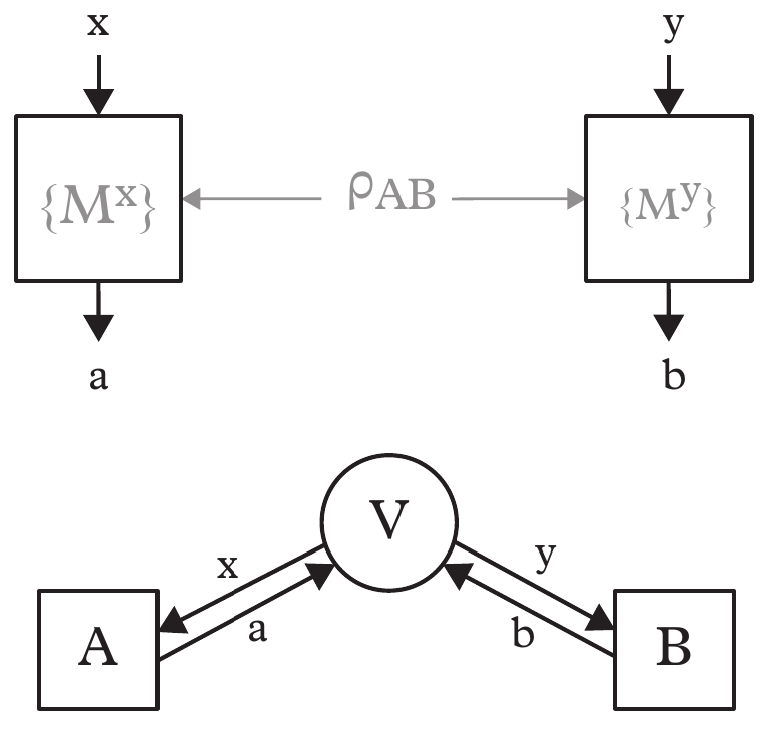
\includegraphics[width=0.5\linewidth]{images/BellScenario.png}
    \caption{Bell scenario. Taken from \cite{BellNonlocality}}
    \label{fig:bell_scenario}
\end{figure}

In each round, before receiving the inputs, the players agree on a process to produce the outcomes. This process is identified by a hidden variable $\lambda$ and is described by a collection of conditional probabilities $P_\lambda(a,b \mid x,y)$:

\[
\mathcal{P}_\lambda = \{ P_\lambda(a,b \mid x,y) \mid a\in \mathcal{A}, b \in \mathcal{B}, x \in \mathcal{X}, y \in \mathcal{Y} \},
\]

\[
P_\lambda (a,b \mid x,y) \geq 0 \quad \forall a\in \mathcal{A}, b \in \mathcal{B}, x \in \mathcal{X}, y \in \mathcal{Y},
\]

\[
\sum_{a\in \mathcal{A}, b\in \mathcal{B}} P_\lambda(a,b \mid x,y) = 1 \quad \forall x \in \mathcal{X}, y\in \mathcal{Y}.
\]

The number of parameters required to describe a process is $D_{\text{gen}} = M_A M_B (m_A m_B - 1)$. A \textbf{deterministic process} is one where the outputs are completely determined by the inputs. The total number of deterministic processes is $\#_{\text{D}} = (m_A m_B)^{M_A M_B}$, because for each pair of inputs we must specify which pair of outcomes is produced.

Two standard assumptions are made:
\begin{itemize}
    \item \textbf{Measurement independence:} the hidden variable $\lambda$ is independent of the inputs $(x,y)$.
    \item \textbf{I.I.D. strategies:} the process in each round is independent and identically distributed, i.e., it does not depend on previous rounds.
\end{itemize}

Since the verifier does not know the process in each round, they observe the following \textbf{behaviour}:

\[
\mathcal{P} = \{ P(a,b \mid x, y) \mid \forall a\in \mathcal{A}, b \in \mathcal{B}, x \in \mathcal{X}, y \in \mathcal{Y}\},
\]

\[
P(a,b \mid x, y) = \int d\lambda \, Q(\lambda) \, P_\lambda(a,b \mid x,y).
\]

If the same deterministic process $\lambda_d$ is used in every round (i.e., $Q(\lambda) = \delta(\lambda - \lambda_d)$), then the behaviour is said to be \textbf{deterministic}.

\subsection{Local behaviours}

A process is called \textbf{local} if it factorises as:

\[
P_\lambda(a,b \mid x,y) \stackrel{\text{LV}}{=} P_\lambda(a \mid x) \, P_\lambda(b \mid y).
\]

A behaviour is \textbf{local} if it can be expressed as a convex combination of local processes. A behaviour that cannot be expressed in this way is called \textbf{non-local}. In a local process, the output of each player in each round is independent of the other player's input.

A \textbf{local deterministic process} is one where, for each input, the output is deterministic:

\[
P_{\text{LD},\lambda}(a \mid x) = \delta_{a, f(x,\lambda)}, \qquad
P_{\text{LD},\lambda}(b \mid y) = \delta_{b, g(y,\lambda)}.
\]

The number of local deterministic processes is:

\[
\#_{\text{LD}} = m_A^{M_A} \, m_B^{M_B}.
\]

\textbf{Fine's theorem:} The following statements are equivalent:
\begin{itemize}
    \item A behaviour $\mathcal{P}$ is local if and only if it can be written as a convex combination of local deterministic processes:
    \[
    P(a,b \mid x,y) \stackrel{\text{LV}}{=} \sum_{j=1}^{m_A^{M_A}} \sum_{k=1}^{m_B^{M_B}} q_{jk} \, \delta_{a, f_j(x)} \, \delta_{b, g_k(y)},
    \]
    where $\lambda = (j,k)$ and $\sum_{j,k} q_{jk} = 1$.

    \item A behaviour $\mathcal{P}$ is local if and only if there exists a joint probability distribution $\boldsymbol{P}(a_1,\dots, a_{M_A}; b_1 , \dots, b_{M_B})$ such that every $P(a,b \mid x,y)$ can be obtained as a marginal:
    \[
    P(a,b \mid x,y) \stackrel{\text{LV}}{=} \sum_{\{a_j \mid j\neq x\}} \sum_{\{b_k \mid k\neq y\}} \boldsymbol{P}(a_1, \dots , a_{M_A}; b_1, \dots, b_{M_B}).
    \]
\end{itemize}

\subsection{Local polytope and Bell inequalities}

Let $\mathcal{P}_{LV1}$ and $\mathcal{P}_{LV2}$ be local behaviours, then:

\[
P_{LV1}(a, b|x, y) \overset{LV}{=} \sum_{j=1}^{m_A^{M_A}} \sum_{k=1}^{m_B^{M_B}} q_{jk} \delta_{a=f_j(x)} \delta_{b=b_k(y)}
\]

\[
P_{LV2}(a, b|x, y) \overset{LV}{=} \sum_{j=1}^{m_A^{M_A}} \sum_{k=1}^{m_B^{M_B}} p_{jk} \delta_{a=f_j(x)} \delta_{b=b_k(y)}
\]


Let $\lambda \in \left[ 0,1 \right]$, then:

\begin{eqnarray*}
    \lambda P_{LV1}(a, b|x, y) + (1-\lambda)P_{LV1}(a, b|x, y) &=& \sum_{j=1}^{m_A^{M_A}} \sum_{k=1}^{m_B^{M_B}} \left[ \lambda q_{jk} \delta_{a=f_j(x)} \delta_{b=b_k(y)} + (1-\lambda)p_{jk}\delta_{a=f_j(x)} \delta_{b=b_k(y)}\right] \\
    &=& \sum_{j=1}^{m_A^{M_A}} \sum_{k=1}^{m_B^{M_B}} \left[ \left(\lambda q_{jk} + (1-\lambda)p_{jk}\right) \delta_{a=f_j(x)} \delta_{b=b_k(y)} \right]
\end{eqnarray*}

The term inside the last parenthesis sums to 1. Therefore, this convex combination is also a local behaviour, which means that the set of local behaviours is a convex set. Since the local deterministic processes cannot be expressed as a convex combination of other local behaviours, this means that the local deterministic processes are the extremal points of the set of all local behaviours $\mathcal{L}$. In the figure \ref{fig:LocalPolytope} is shown the local polytope $\mathcal{L}$, the quantum set $\mathcal{Q}$ and the no-signaling polytope $\mathcal{NS}$.

\begin{figure}[H]
    \centering
    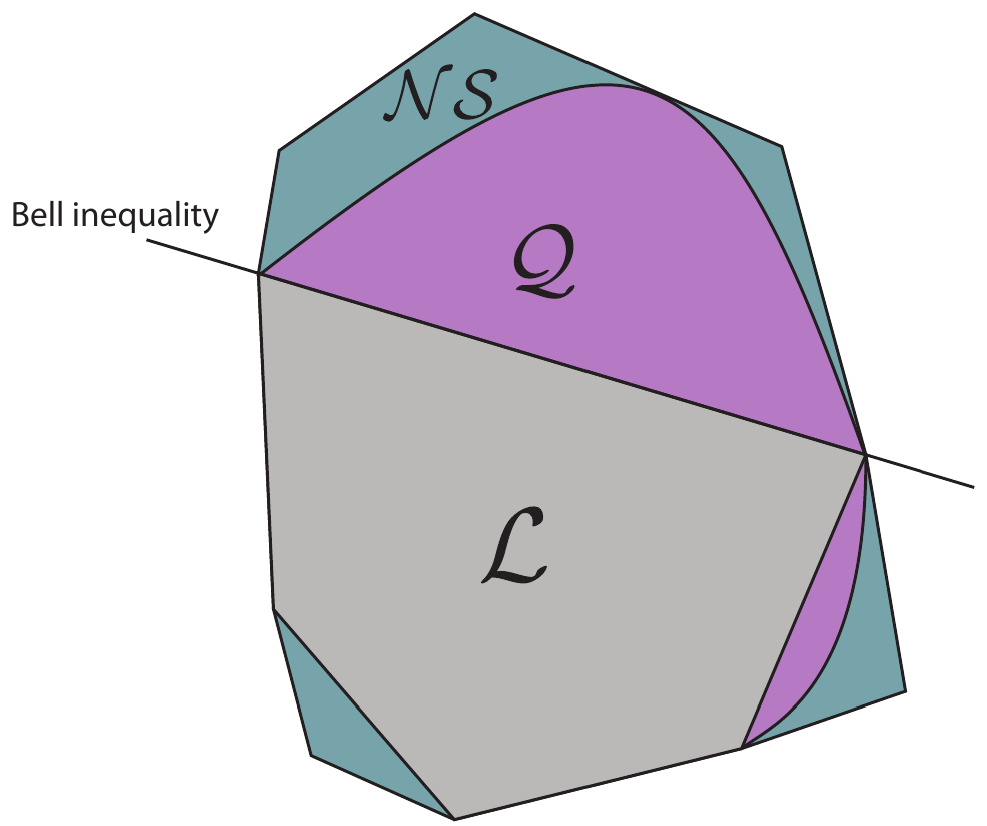
\includegraphics[width=0.5\linewidth]{images/LocalPolytope.png}
    \caption{Taken from \cite{PaperBellNonlocality}}
    \label{fig:LocalPolytope}
\end{figure}

\newpage
\section{CHSH Inequality}

\subsection{CHSH game}

The CHSH game is a bipartite Bell scenario. Let Alice and Bob be the players, who are spatially separated. The referee $R$ chooses two bits $x$ and $y$ uniformly at random and sends them to Alice and Bob respectively. Alice and Bob cannot communicate with each other; they send back two bits $a$ and $b$ to the referee. Locality implies that $a$ is independent of $y$ while $b$ is independent of $x$. Once the referee receives the outcomes, it evaluates the logical proposition:

\[
x \land y = a \oplus b,
\]

where $\land$ denotes the logical AND and $\oplus$ denotes addition modulo 2.

Let $V(x,y,a,b)$ be the indicator function for the winning condition:

\[
V(x,y,a,b) = \begin{cases}
    1, & \text{if } x \land y = a \oplus b,\\[2pt]
    0, & \text{otherwise}.
\end{cases}
\]

If $V(x,y,a,b)=1$, they win the round; otherwise, they lose. Let $p_{AB|XY}(a,b|x,y)$ be the conditional probability distribution of the strategy used by Alice and Bob. Since the referee's bits are uniformly distributed, $p_{XY}(x,y)=1/4$. Hence the winning probability is

\[
\frac{1}{4}\sum_{a,b,x,y} V(x,y,a,b) \, p_{AB|XY}(a,b|x,y).
\]

Assume that there is a random variable $\Lambda$ taking values $\lambda$, which describes either a classical or a quantum strategy. By the law of total probability,

\[
p_{AB|XY}(a,b|x,y) = \int d\lambda \; p_{AB|\Lambda XY}(a,b|\lambda,x,y) \; p_{\Lambda|XY}(\lambda|x,y).
\]

\subsection{Classical strategy}

In the classical case, $\Lambda$ corresponds to the classical correlations that Alice and Bob share before the game starts. Therefore

\[
p_{\Lambda|XY}(\lambda|x,y) = p_\Lambda(\lambda).
\]

Because Alice and Bob are far apart, their outcomes are independent. Moreover, classical strategies enforce local correlations: Alice's outcome $a$ is independent of Bob's input $y$, and Bob's outcome $b$ is independent of Alice's input $x$. Hence

\[
p_{AB|\Lambda XY}(a,b|\lambda,x,y) = p_{A|\Lambda XY}(a|\lambda,x,y) \, p_{B|\Lambda XY}(b|\lambda,x,y)
= p_{A|\Lambda X}(a|\lambda,x) \, p_{B|\Lambda Y}(b|\lambda,y).
\]

Figure~\ref{fig:CHSH_classical} illustrates the assumptions used to obtain this factorization.

\begin{figure}[H]
    \centering
    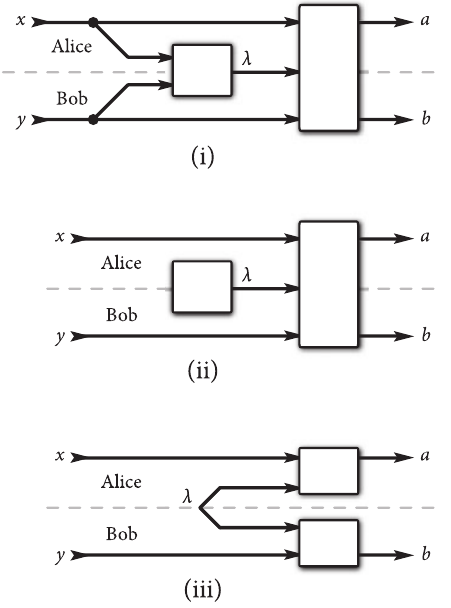
\includegraphics[width=0.4\linewidth]{images/CHSH_classical.png}
    \caption{Reductions of the conditional probability $p_{AB|\Lambda XY}$ under the assumptions of a classical strategy in the CHSH game: (i) arbitrary strategy (where $\Lambda$ could depend on $X$ and $Y$), (ii) requiring $\Lambda$ to be independent of $X$ and $Y$, and (iii) imposing locality. Taken from \cite{QIT}.}
    \label{fig:CHSH_classical}
\end{figure}

Therefore the conditional probability distribution becomes

\[
p_{AB|XY}(a,b|x,y) = \int d\lambda \; p_\Lambda(\lambda) \; p_{A|\Lambda X}(a|\lambda,x) \; p_{B|\Lambda Y}(b|\lambda,y).
\]

The stochastic maps $p_{A|\Lambda X}$ and $p_{B|\Lambda Y}$ can be expressed as convex combinations of deterministic binary-valued functions. For any such map there exist local random variables $N$ and $M$ and deterministic functions $f$ and $g$ such that

\begin{eqnarray*}
    p_{A|\Lambda X}(a|\lambda,x) &=& \int dn \; p_N(n) \; f(a|\lambda,x,n),\\
    p_{B|\Lambda Y}(b|\lambda,y) &=& \int dm \; p_M(m) \; g(b|\lambda,y,m).
\end{eqnarray*}

Substituting these representations yields

\[
p_{AB|XY}(a,b|x,y) = \int d\lambda \, dn \, dm \; p_\Lambda(\lambda)\, p_N(n)\, p_M(m) \; f(a|\lambda,x,n) \; g(b|\lambda,y,m).
\]

Since $N$ and $M$ are local random variables, they can be absorbed into $\Lambda$ without loss of generality. Consequently,

\[
p_{AB|XY}(a,b|x,y) = \int d\lambda \; p_\Lambda(\lambda) \; f'(a|\lambda,x) \; g'(b|\lambda,y),
\]

where $f'$ and $g'$ are deterministic response functions.

Inserting this expression into the winning probability gives

\begin{eqnarray*}
    \frac{1}{4}\sum_{a,b,x,y}V(x,y,a,b) \, p_{AB|XY}(a,b|x,y)
    &=& \frac{1}{4}\sum_{a,b,x,y}V(x,y,a,b) \int d\lambda \, p_\Lambda(\lambda) \, f'(a|\lambda,x) \, g'(b|\lambda,y) \\
    &=& \int d\lambda \, p_\Lambda(\lambda) \left[ \frac{1}{4}\sum_{a,b,x,y} V(x,y,a,b) \, f'(a|\lambda,x) \, g'(b|\lambda,y) \right] \\
    &\leq& \frac{1}{4}\sum_{a,b,x,y} V(x,y,a,b) \, f'(a|\lambda^*,x) \, g'(b|\lambda^*,y),
\end{eqnarray*}

where $\lambda^*$ is the value that maximizes the expression inside the brackets. This shows that it suffices to consider deterministic processes to obtain an upper bound on the classical winning probability.

In a deterministic classical strategy, Alice chooses a bit $a_x$ depending only on her input $x$, and Bob chooses $b_y$ depending only on his input $y$. The following table enumerates all four possible pairs of inputs:

\begin{center}
    \begin{tabular}{|c|c|c|c|}
        \hline
        $x$ & $y$ & $x \land y$ & $a_x \oplus b_y$ \\
        \hline
        0 & 0 & 0 & $a_0 \oplus b_0$ \\
        0 & 1 & 0 & $a_0 \oplus b_1$ \\
        1 & 0 & 0 & $a_1 \oplus b_0$ \\
        1 & 1 & 1 & $a_1 \oplus b_1$ \\
        \hline
    \end{tabular}
\end{center}

Suppose they could win in every round, i.e., $x \land y = a_x \oplus b_y$ for all four rows. Summing the left‑hand column ($x \land y$) modulo 2 gives $0+0+0+1 = 1$. Summing the right‑hand column ($a_x \oplus b_y$) modulo 2 gives $0$ because each term $a$ and $b$ appears twice, so the total is $0$ (since $a_0\oplus b_0 \oplus a_0\oplus b_1 \oplus a_1\oplus b_0 \oplus a_1\oplus b_1 = 0$). This is a contradiction, because the two sums cannot be unequal if the equality holds row‑wise. Hence it is impossible to satisfy all four conditions simultaneously. At most three of them can be satisfied by any deterministic classical strategy. Consequently, the maximum winning probability for any classical strategy is bounded by

\[
\frac{1}{4}\sum_{a,b,x,y} V(x,y,a,b) \, p_{AB|XY}(a,b|x,y) \le \frac{3}{4}.
\]

\subsection{Quantum strategy}

In this case, the shared resource $\lambda$ is given by the shared quantum state $|\phi\rangle_{AB}$. Alice and Bob perform certain measurements according to the bits they receive. Let $\{ \Pi_a^{(x)} \}$ Alice's x-dependent measurement and $\{ \Pi_b^{(y)} \}$ be Bob's y-dependent measurement, such that they satisfy:

\[
\sum_a \Pi_a^{(x)} = \sum_b \Pi_b^{(y)} = \mathbb{I}.
\]

The conditional probability distribution is given by:

\[
p_{AB|XY}(a,b | x,y) = \langle \phi |_{AB} \Pi_a^{(x)} \otimes \Pi_b^{(y)} | \phi \rangle_{AB},
\]

then, the winning probability for a quantum strategy is given by:

\[
\frac{1}{4}\sum_{a,b,x,y} V(x,y,a,b)\langle \phi |_{AB} \Pi_a^{(x)} \otimes \Pi_b^{(y)} | \phi \rangle_{AB}
\]

For the CHSH game, $\cos^2(\pi/8) \approx 0.85$ is the maximum winning probability that can be achieved through a quantum strategy. This result is known as the \textbf{Tsirelson's bound}.\\

If $(x,y) \in \{ (0,0), (0,1), (1,0) \}$, then, it must hold that $a=b$ so Alice and Bob can win. Since $\{ \Pi_a^{(x)} \}$ and $\{ \Pi_b^{(y)} \}$ are measurements that depend on the input bits, they constitute the strategy that Alice and Bob agree before starting the game. The winning probability and losing probabilites in this case are given by:

\begin{eqnarray*}
    \text{Winning probability:} &=& \langle \phi|_{AB} \Pi_0^{(x)} \otimes \Pi_0^{(y)} | \phi \rangle_{AB} + \langle \phi|_{AB} \Pi_1^{(x)} \otimes \Pi_1^{(y)} | \phi \rangle_{AB} \\
    \text{Losing probability:} &=& \langle \phi|_{AB} \Pi_0^{(x)} \otimes \Pi_1^{(y)} | \phi \rangle_{AB} + \langle \phi|_{AB} \Pi_1^{(x)} \otimes \Pi_0^{(y)} | \phi \rangle_{AB}
\end{eqnarray*}

Let $A^{(x)} = \Pi_0^{(x)} - \Pi_1^{(x)}$ and $B^{(y)} = \Pi_0^{(y)} - \Pi_1^{(y)}$. The winning probability minus the losing probability is:

\[
\langle \phi|_{AB} A^{(x)} \otimes B^{(y)} | \phi \rangle_{AB}
\]

Now, if $(x,y) = (1,1)$, it must hold that $a\neq b$ so Alice and Bob can win. Therefore, the winning and losing probabilities are the following:
\begin{eqnarray*}
    \text{Winning probability:} &=& \langle \phi|_{AB} \Pi_0^{(1)} \otimes \Pi_1^{(1)} | \phi \rangle_{AB} + \langle \phi|_{AB} \Pi_1^{(1)} \otimes \Pi_0^{(1)} | \phi \rangle_{AB} \\
    \text{Losing probability:} &=& \langle \phi|_{AB} \Pi_0^{(1)} \otimes \Pi_0^{(1)} | \phi \rangle_{AB} + \langle \phi|_{AB} \Pi_1^{(1)} \otimes \Pi_1^{(1)} | \phi \rangle_{AB}
\end{eqnarray*}

Then, the probability of winning minus the probability of losing is:

\[
-\langle \phi|_{AB} A^{(1)} \otimes B^{(1)} | \phi \rangle_{AB}
\]

Taking into account that the probability distributions of the inputs is uniformly random, it follows that when averaging over all of the input bits, the probability of winning minus the probability of losing is given by:

\[
\frac{1}{4}\langle \phi|_{AB} C_{AB} | \phi \rangle_{AB},
\]

where $C_{AB}$ is the CHSH operator, defined as:

\[
C_{AB} = A^{(0)} \otimes B^{(0)} + A^{(0)} \otimes B^{(1)} + A^{(1)} \otimes B^{(0)} - A^{(1)} \otimes B^{(1)}
\]

Let's compute $C_{AB}^2$:

\begin{eqnarray*}
    C_{AB}^2 &=& A^{(0)}A^{(0)} \otimes B^{(0)}B^{(0)} + A^{(0)}A^{(0)} \otimes B^{(1)}B^{(1)} + A^{(1)}A^{(1)} \otimes B^{(0)}B^{(0)} + A^{(1)}A^{(1)} \otimes B^{(1)}B^{(1)} \\
    && + A^{(0)}A^{(0)} \otimes B^{(0)}B^{(1)} + A^{(0)}A^{(1)} \otimes B^{(0)}B^{(0)} - A^{(0)}A^{(1)} \otimes B^{(0)}B^{(1)} + A^{(0)}A^{(0)} \otimes B^{(1)}B^{(0)} \\
    && + A^{(0)}A^{(1)} \otimes B^{(1)}B^{(0)} - A^{(0)}A^{(1)} \otimes B^{(1)}B^{(1)} + A^{(1)}A^{(0)} \otimes B^{(0)}B^{(0)} + A^{(1)}A^{(0)} \otimes B^{(0)}B^{(1)} \\
    && - A^{(1)}A^{(1)} \otimes B^{(0)}B^{(1)} - A^{(1)}A^{(0)} \otimes B^{(1)}B^{(0)} - A^{(1)}A^{(0)} \otimes B^{(1)}B^{(1)} - A^{(1)}A^{(1)} \otimes B^{(1)}B^{(0)},\\
    &=& 4\mathbb{I}_{AB} - \left[ A^{(0)}, A^{(1)} \right] \otimes \left[ B^{(0)}, B^{(1)} \right].
\end{eqnarray*}

Let's compute the infinity norm of $C_{AB}^2$, that is it's largest eigenvalue. We must take into account the following properties of this norm:

\begin{eqnarray*}
    \Vert cR \Vert_\infty &=& |c| \Vert R \Vert_\infty \\
    \Vert RS \Vert_\infty &\leq& \Vert R \Vert_\infty \Vert S \Vert_\infty \\
    \Vert R + S \Vert_\infty &\leq& \Vert R \Vert_\infty + \Vert S \Vert_\infty
\end{eqnarray*}

\begin{eqnarray*}
    \Vert C_{AB}^2\Vert_{\infty} &=&  \left|\left| 4\mathbb{I}_{AB} - \left[ A^{(0)}, A^{(1)} \right] \otimes \left[ B^{(0)}, B^{(1)} \right] \right|\right|_\infty \\
    &\leq& 4 \Vert \mathbb{I}_{AB}\Vert_\infty + \left|\left| \left[ A^{(0)}, A^{(1)} \right] \otimes \left[ B^{(0)}, B^{(1)} \right] \right|\right|_\infty \\
    &=& 4 + \left|\left| \left[ A^{(0)}, A^{(1)} \right] \right|\right|_\infty + \left|\left| \left[ B^{(0)}, B^{(1)} \right] \right|\right|_\infty \\
    &\leq& 4 + 2\cdot 2 = 8
\end{eqnarray*}

This implies that:

\[
\Vert C_{AB} \Vert_\infty \leq \sqrt{8} = 2\sqrt{2}.
\]

Therefore, the probability of winning minus the probability of losing is bounded by:

\[
\frac{1}{4}\Vert C_{AB}\Vert_\infty \leq \frac{\sqrt{2}}{2},
\]

for any quantum strategy. Since the probability of winning $W$ plus the probability of losing $L$ is 1, we have the following:

\begin{eqnarray*}
    W - L &\leq& \frac{\sqrt{2}}{2}, \\
    W + L &=& 1.
\end{eqnarray*}

Then, the winning probability is bounded for any quantum strategy by the Tsirelson's bound:

\[
W \leq \frac{1+\sqrt{2}/2}{2} = \frac{2 + \sqrt{2}}{4} = \cos^2\left( \frac{\pi}{8} \right).
\]


\newpage
\section{CGLMP Inequalities}

Just as the CHSH inequality provides a certification of entanglement in bipartite 2-dimensional systems, the family of CGLMP inequalities provide thir certification for bipartite qudit system. Let $A_1$ and $A_2$ be Alice's measurements and $B_1$ and $B_2$ be Bob's measurements, where each of these measurements has $d$ possible outcomes.\\

A local hidden variable theory (LHVT) is described by $d^4$ probabilities $c_{jklm}$ $(j,k,l,m = 0,\dots, d-1)$, where $j$, $k$, $l$ and $m$ correspond to the measurement outcomes of $A_1$, $A_2$, $B_1$ and $B_2$ respectively. Assuming that these values are well defined comes from a realistic theory. In this case, Alice and Bob's strategy is deterministic.
\[
\sum_{j,k,l,m} c_{jklm} = 1 \quad , \quad c_{jklm} \geq 0.
\]

The joint probabilities are given by:

\begin{eqnarray*}
    P(A_1 = j, B_1=l) &=& \sum_{k,m} c_{jklm} \\
    P(A_1 = j, B_2=m) &=& \sum_{k,l} c_{jklm} \\
    P(A_2 = k, B_1=l) &=& \sum_{j,m} c_{jklm} \\
    P(A_2 = k, B_2=m) &=& \sum_{j,l} c_{jklm} 
\end{eqnarray*}

Given a choice of local variables $j,k,l,m$, lt's define the following new variables:

\begin{eqnarray*}
    r' &=& B_1 - A_1 = l - j \\
    s' &=& A_2 - B_1 = k - l \\
    t' &=& B_2 - A_2 = m - k \\
    u' &=& A_1 - B_2 = j - m \\
\end{eqnarray*}

It can be seen that $r'+s'+t'+u'=0$, which applies a constraint on this variables. If three of these variables are determined, the other one is inmediately determined by this constraint, so the system only has three degrees of freedom instead of four.\\

Let's consider the following Bell expression:

\begin{equation}
    I = P(A_1 = B_1) + P(B_1 = A_2 + 1) + P(A_2 = B_2) + P(B_2 = A_1),
    \label{eq:CGLMP1}
\end{equation}

where
\[
P(A_a = B_b + k) = \sum_{j=0}^{d-1} P(A_a = j, B_b = j + k \mod d)
\]

Given the restriction for the variables $r', s', t', u'$ because of the local realism assumption, at least $3$ of the $4$ probabilities in the expression \ref{eq:CGLMP1} can be attained. For nonlocal correlations, it is possible to attain $I = 4$.

\newpage
\section{Quantifiers of Entanglement and Measurement Incompatibility}

\subsection{Entanglement quantifier}

A quantum bipartite pure state $|\Psi\rangle_{AB}$ is \textbf{entangled} if it cannot be expressed as a tensor product between a state $|\psi\rangle_A \in \mathcal{H}_A$ and $|\phi\rangle_B \in \mathcal{H}_B$, that is:
\[
|\Psi\rangle_{AB} \neq |\psi \rangle_{A} \otimes |\phi \rangle_B
\]

For mixed bipartite systems, a quantum state $\rho_{AB}$ is \textit{entangled} if and only if cannot be written as a convex combination of product states:
\[
\rho_{AB} \neq \sum_\lambda p_\lambda \rho_\lambda^A \otimes \rho_\lambda^B
\]

The problem of determining if a state is entangled or not is a NP-hard problem in the sense that it doesn't exist an efficient algorithm that can determine this.\\

Let $X_{AB} \in \mathcal{H}_{AB} = \mathcal{H}_A \otimes \mathcal{H}_B$ and let $\{ |i\rangle\}$ be an orthonormal basis for $\mathcal{H}_B$. The \textbf{partial transpose} is defined as:
\[
X_{AB}^{T_A} = \sum_{i,j} (|j\rangle \langle i | \otimes \mathbb{I}) X_{AB} (|j\rangle \langle i | \otimes \mathbb{I})
\]

The \textit{positive-partial transpose} criterion states that if the partial transpose of a quantum state $\rho_{AB}$ isn't semidefinite positive, then $\rho_{AB}$ is entangled, that is:
\[
\rho_{AB}^{T_A} \not\succeq 0 \longrightarrow \rho_{AB} \neq \sum_\lambda p_\lambda \rho_\lambda^A \otimes \rho_\lambda^B
\]

The set of entangled states can be classified between PPT and NPT according if they are positive or negative partial transpose respectively. Because there are entangled states that belong to the PPT set, it cannot be stablished anything about the separability of a PPT state. Let $S_{PPT}$ be the set of positive partial transpose states, and $S_{sep}$ the set of separable states (not entangled), then:
\[
S_{sep} \subseteq S_{PPT}.
\]

A measure of the "negativity" of an operator is the absolute value of the sum of it's negative eigenvalues. Let $A$ be an hermitian operator, then:
\[
A = A^{(+)} - A^{(-)},
\]

where $A^{(+)}, A^{(-)} \succeq 0$. The positive eigenvalues and it's correspondent eigenprojectors form $A^{(+)}$ while the absolute value of the negative eigenvalues and their correspondent eigenprojectors form $A^{(-)}$. The \textit{negativity} of $A$ is defined as:
\[
\mathcal{N}(A) = ||A^{-}||_1 = \sum_{\lambda < 0}|\lambda|
\]

Then, the \textbf{negativity of entanglement} can be cast as the following SDP:

\begin{eqnarray*}
    \mathcal{N}(\rho_{AB}) = \text{Minimise} && \operatorname{tr}(\textcolor{red}{Y}), \\
    \text{constrained to} && \rho_{AB}^{T_A} = \textcolor{red}{Z} - \textcolor{red}{Y}, \\
    && \textcolor{red}{Y}, \textcolor{red}{Z} \succeq 0.
\end{eqnarray*}

The dual formulation of this SDP is the following:

\begin{eqnarray*}
    \mathcal{N}(\rho_{AB}) = \text{Maximise} && -\operatorname{tr}(\textcolor{red}{X}^{T_A}\rho_{AB}), \\
    \text{constrained to} && \mathbb{I} \succeq \textcolor{red}{X}, \\
    && \textcolor{red}{X} \succeq 0.
\end{eqnarray*}

The operator $\textcolor{red}{W}$ is known as an \textbf{entanglement witness}.
\begin{eqnarray*}
    \mathcal{N}(\rho_{AB}) = \text{Maximise} && -\operatorname{tr}(\textcolor{red}{W}\rho_{AB}) \\
        \text{constrained to} && \mathbb{I} \succeq \textcolor{red}{W}^{T_A}, \quad \textcolor{red}{W}^{T_A} \succeq 0.
\end{eqnarray*}

Let $\sigma_{AB}$ be a separable state. Since $\textcolor{red}{W}^{T_A}, \sigma_{AB}^{T_A} \succeq 0$, it follows:
\[
\operatorname{tr}(\textcolor{red}{W}^{T_A} \sigma_{AB}^{T_A}) = \operatorname{tr}(\textcolor{red}{W}\sigma_{AB}) \geq 0.
\] 

Therefore, if $\operatorname{tr}(\textcolor{red}{W}\rho_{AB}) \leq 0$, it follows that $\rho_{AB}$ is entangled. However, \textit{entanglement witnesses} are only able to detect NPT entangled states.\\

Another quantifier of entanglement is the \textbf{random robustness of entanglement}, which can be interpreted as the minimum amount of noise required to make a state into a separable one. It is defined as the following optimization problem:
\begin{eqnarray*}
        R_R(\rho_{AB}) = \text{Minimise} && \textcolor{red}{r}, \\
        \text{constrained to} && \frac{\rho_{AB} + \textcolor{red}{r}\frac{\mathbb{I}_A \otimes \mathbb{I}_B}{d_A d_B}}{1 + \textcolor{red}{r}} \in S_{sep}, \\
        && \textcolor{red}{r} \geq 0.
\end{eqnarray*}

Since it doesn't exist an efficient algorithm in order to determine if a state is separable or not, it may be useful to relax this problem given some other criterion.\\

Given the the PPT criterion, the \textit{random robustness of entanglement} can be relaxed into $R_R^{NPT}(\rho_{AB})$, which is the minimum amount of noise required to make a state into a PPT state, that is the following SDP:
\begin{eqnarray*}
    R_R^{NPT}(\rho_{AB}) = \text{Minimise} && \textcolor{red}{r} \\
    \text{constrained to} && \left( \rho_{AB} + \textcolor{red}{r}\frac{\mathbb{I}_A \otimes \mathbb{I}_B}{d_A d_B} \right)^{T_A} \succeq 0,\\
    && \textcolor{red}{r} \geq 0.
\end{eqnarray*}

If $R_R^{NPT}(\rho_{AB}) > 0$, then $\rho_{AB}$ is entangled. Since $S_{sep} \subseteq S_{PPT}$, the optimal value of this SDP lower bound the original problem $R_R^{NPT}(\rho_{AB}) \leq R_R(\rho_{AB})$.


\subsection{Measurement incompatibility quantifier}

For projective measurements, the conmutator between the observables being measured provide a notion of compatibility between their correspondent measurements. For generalized measurements POVM, there exists a more general notion of incompatibility known as \textbf{non-joint measurability}.\\

Let $\{ \mathbb{M}_x \}_x$ be a set of $m$ measurements where each of this measurements is specified by $o$ elements of POVM, such that $\mathbb{M}_x = \{ M_{a|x} \}_a$.\\

The set of measurements $\{ \mathbb{M}_x \}_x$ is \textbf{compatible} if there exists a \textbf{parent measurement} $\textcolor{red}{\mathbb{N}} = \{ \textcolor{red}{N_\lambda}\}$ and a conditional probability distribution $\textcolor{red}{p(a|\lambda, x)}$ such that the statistics of the individual measurements can be recovered given the outcome of the parent measurement, that is:

\[
M_{a|x} = \sum_\lambda \textcolor{red}{p(a|\lambda, x)N_\lambda}
\]

Let $\vec{a} = \left(a_1, \dots a_m \right)$ be the outcomes of the $m$ individual measurements $\{ \mathbb{M}_x\}_x$, $x=1, \dots, m$. Given the outcome $\lambda$ of the parent measurement, the probability of obtaining the oucomes $\vec{a}$ is the following:
\[
\textcolor{red}{p(\vec{a}|\lambda)} = \prod_{x=1}^{m}\textcolor{red}{p(a_x | \lambda, x)}.
\]

Then, the probability that the $x$th component is equal to $a$ is:
\[
\textcolor{red}{p(a|\lambda, x)} = \sum_{\vec{a}} \delta_{a_x, a}\textcolor{red}{p(\vec{a}|\lambda)}.
\]

\begin{eqnarray*}
    M_{a|x} &=& \sum_\lambda \textcolor{red}{p(a|\lambda, x)N_\lambda}, \\
    &=& \sum_{\lambda} \sum_{\vec{a}} \delta_{a_x, a}\textcolor{red}{p(\vec{a}|\lambda) N_\lambda} ,\\
    &=& \sum_{\vec{a}} \delta_{a_x, a}\textcolor{red}{N'_{\vec{a}}},
\end{eqnarray*}

where

\[
\textcolor{red}{N'_{\vec{a}}} = \sum_\lambda \textcolor{red}{p(\vec{a}|\lambda)N_\lambda}\quad , \quad \sum_{\vec{a}}\textcolor{red}{N'_{\vec{a}}} = \mathbb{I}
\]

Therefore, $\textcolor{red}{\mathbb{N}'} = \{ \textcolor{red}{N'_{\vec{a}}} \}_{\vec{a}}$ is a valid measurement. This measurement is known as \textbf{canonical parent measurement}, which has $o^m$ outcomes. The \textit{joint-measurability} problem can be cast as the following feasability SDP:
\begin{eqnarray*}
    \text{Find} && \textcolor{red}{\mathbb{N}}, \\
    \text{constrained to} && M_{a|x} = \sum_{\vec{a}} \delta_{a_x,a}\textcolor{red}{N_{\vec{a}}}, \\
    && \textcolor{red}{N_{\vec{a}}} \succeq 0, \\
    && \sum_{\vec{a}} \textcolor{red}{N_{\vec{a}}} = \mathbb{I}.
\end{eqnarray*}

In order to quantify the incompatibility between the set of measurements, the \textbf{random robustness of measurement incompatibility} is defined as the noise required to make the set of measurements \textit{jointly-measurable}:
\begin{eqnarray*}
    \text{Minimse} && \textcolor{red}{r} \\
    \text{constrained to} && \frac{M_{a|x} + \textcolor{red}{r}\frac{\mathbb{I}}{d}}{1 + \textcolor{red}{r}} = \sum_{\vec{a}} \delta_{a_x, a} \textcolor{red}{N_{\vec{a}}},\quad \forall a,x,\\
    && \textcolor{red}{N_{\vec{a}}} \succeq 0, \quad \forall\vec{a},\\
    && \sum_{\vec{a}}\textcolor{red}{N_{\vec{a}}} = \mathbb{I}, \quad \textcolor{red}{r} \geq 0.
\end{eqnarray*}

This problem can be cast as the following SDP:
\begin{eqnarray*}
    \text{Minimise} && \textcolor{red}{r} \\
    \text{constrained to} && M_{a|x} + \textcolor{red}{r}\frac{\mathbb{I}}{d} = \sum_{\vec{a}}\delta_{a_x,a}\textcolor{red}{N_{\vec{a}}}, \quad \forall a,x,\\
    && \textcolor{red}{N_{\vec{a}}} \succeq 0, \quad \forall\vec{a}, \\
    && \sum_{\vec{a}} \textcolor{red}{N_{\vec{a}}} = (1 + \textcolor{red}{r})\mathbb{I}, \quad \textcolor{red}{r} \geq 0.
\end{eqnarray*}

\newpage
\section{Results}

\begin{figure}[H]
    \centering
    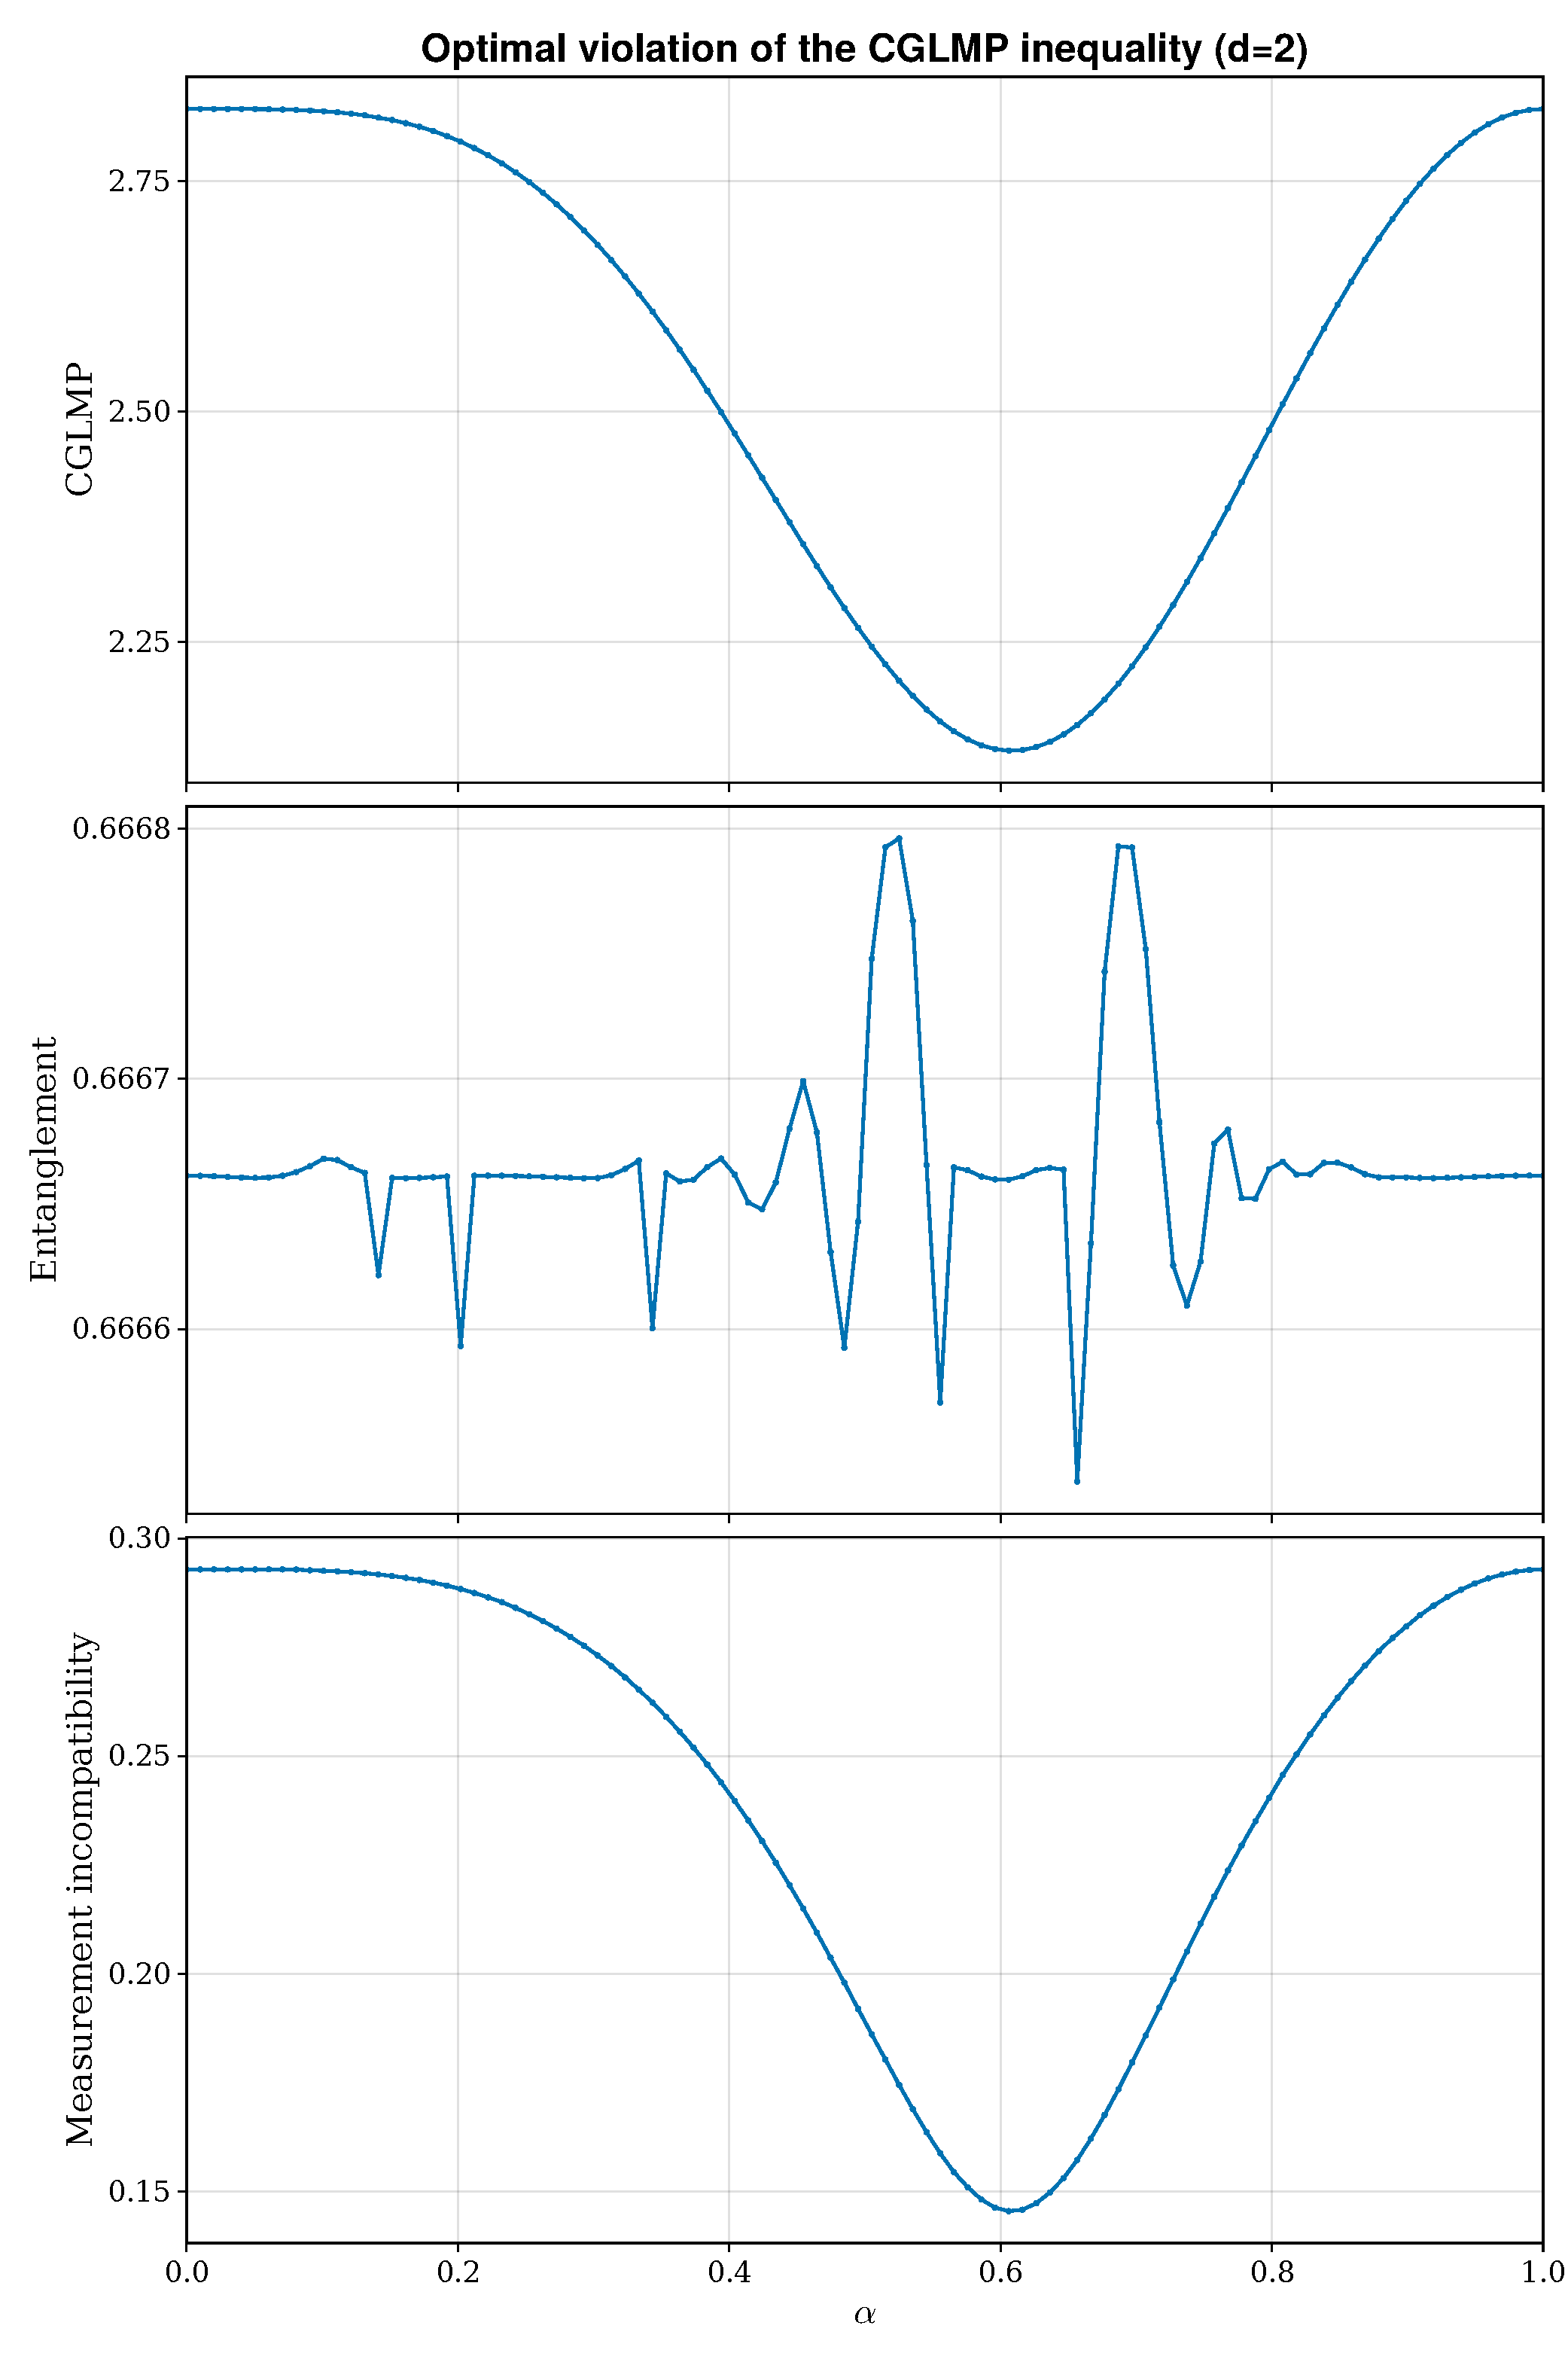
\includegraphics[width=0.6\linewidth]{resultsCGLMP/cglmp_d2.pdf}
    \caption{CGLMP inequality violation for $d=2$, and entanglement and measurement incompatibility quantifiers.}
    \label{fig:CGLMP_d2}
\end{figure}

\begin{figure}[H]
    \centering
    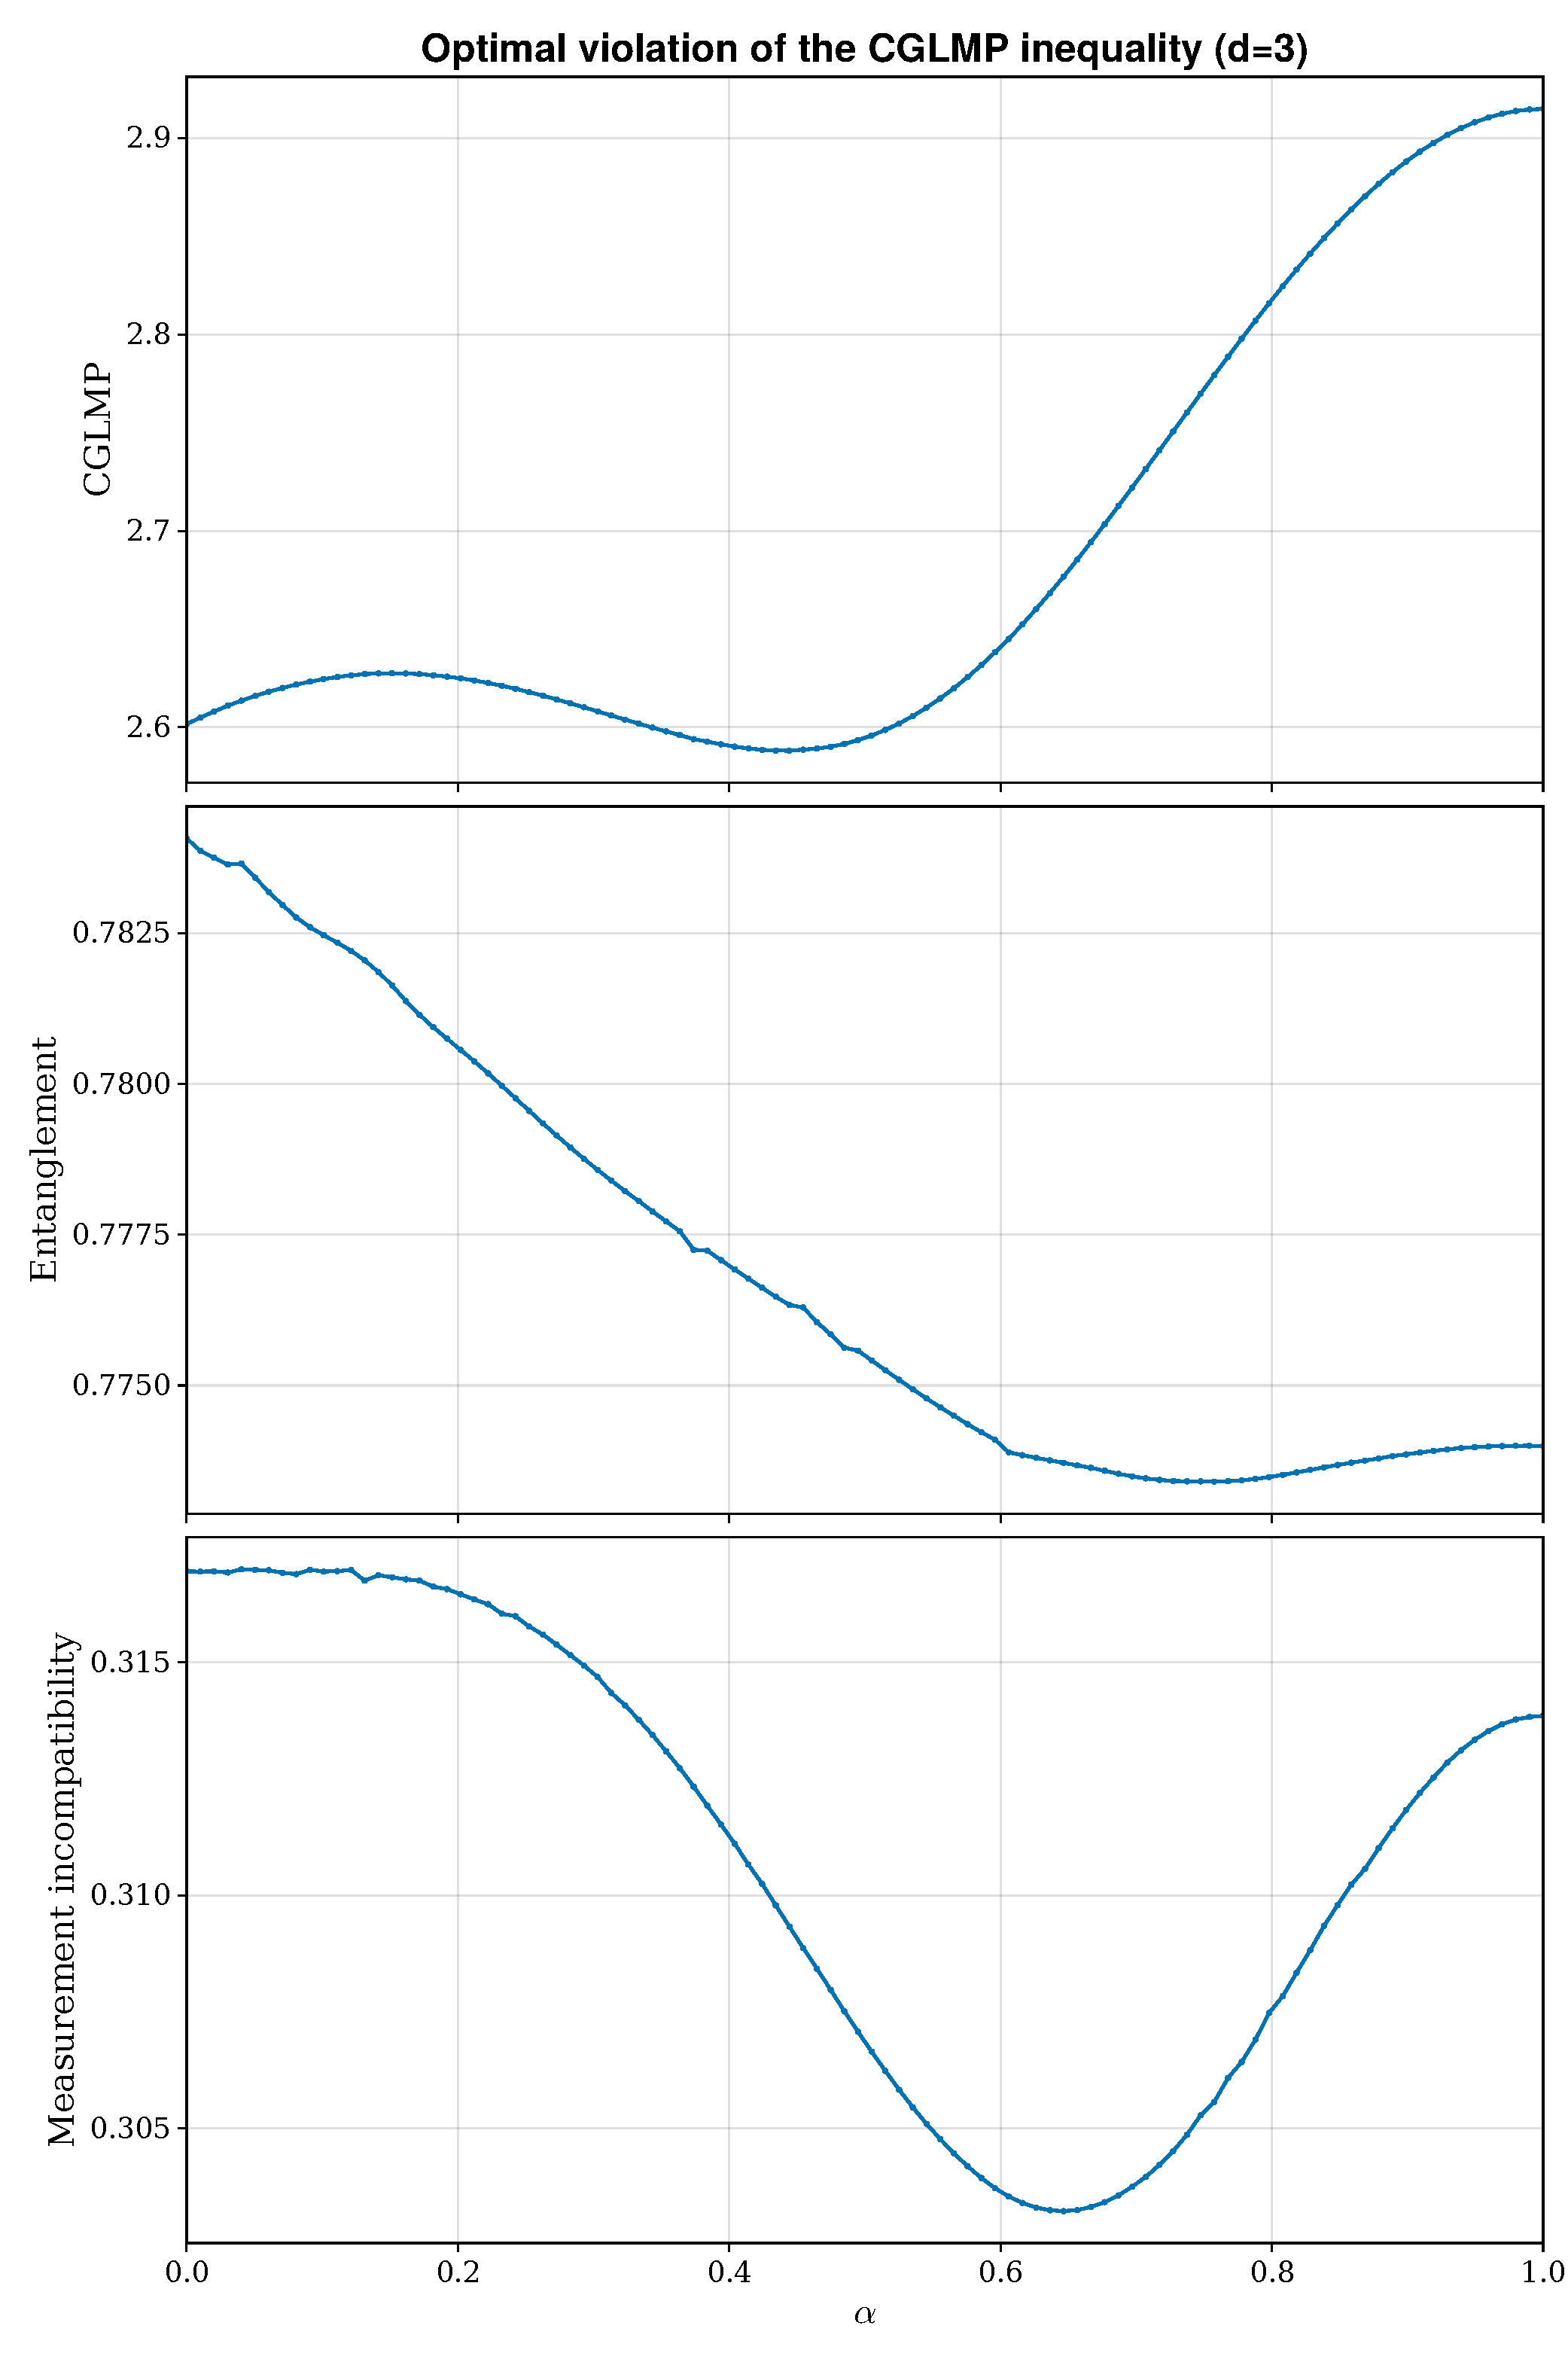
\includegraphics[width=0.6\linewidth]{resultsCGLMP/cglmp_d3.pdf}
    \caption{CGLMP inequality violation for $d=3$, and entanglement and measurement incompatibility quantifiers.}
    \label{fig:CGLMP_d3}
\end{figure}

\begin{figure}[H]
    \centering
    \includegraphics[width=0.6\linewidth]{resultsCGLMP/cglmp_d4.pdf}
    \caption{CGLMP inequality violation for $d=4$, and entanglement and measurement incompatibility quantifiers.}
    \label{fig:CGLMP_d4}
\end{figure}

\begin{figure}[H]
    \centering
    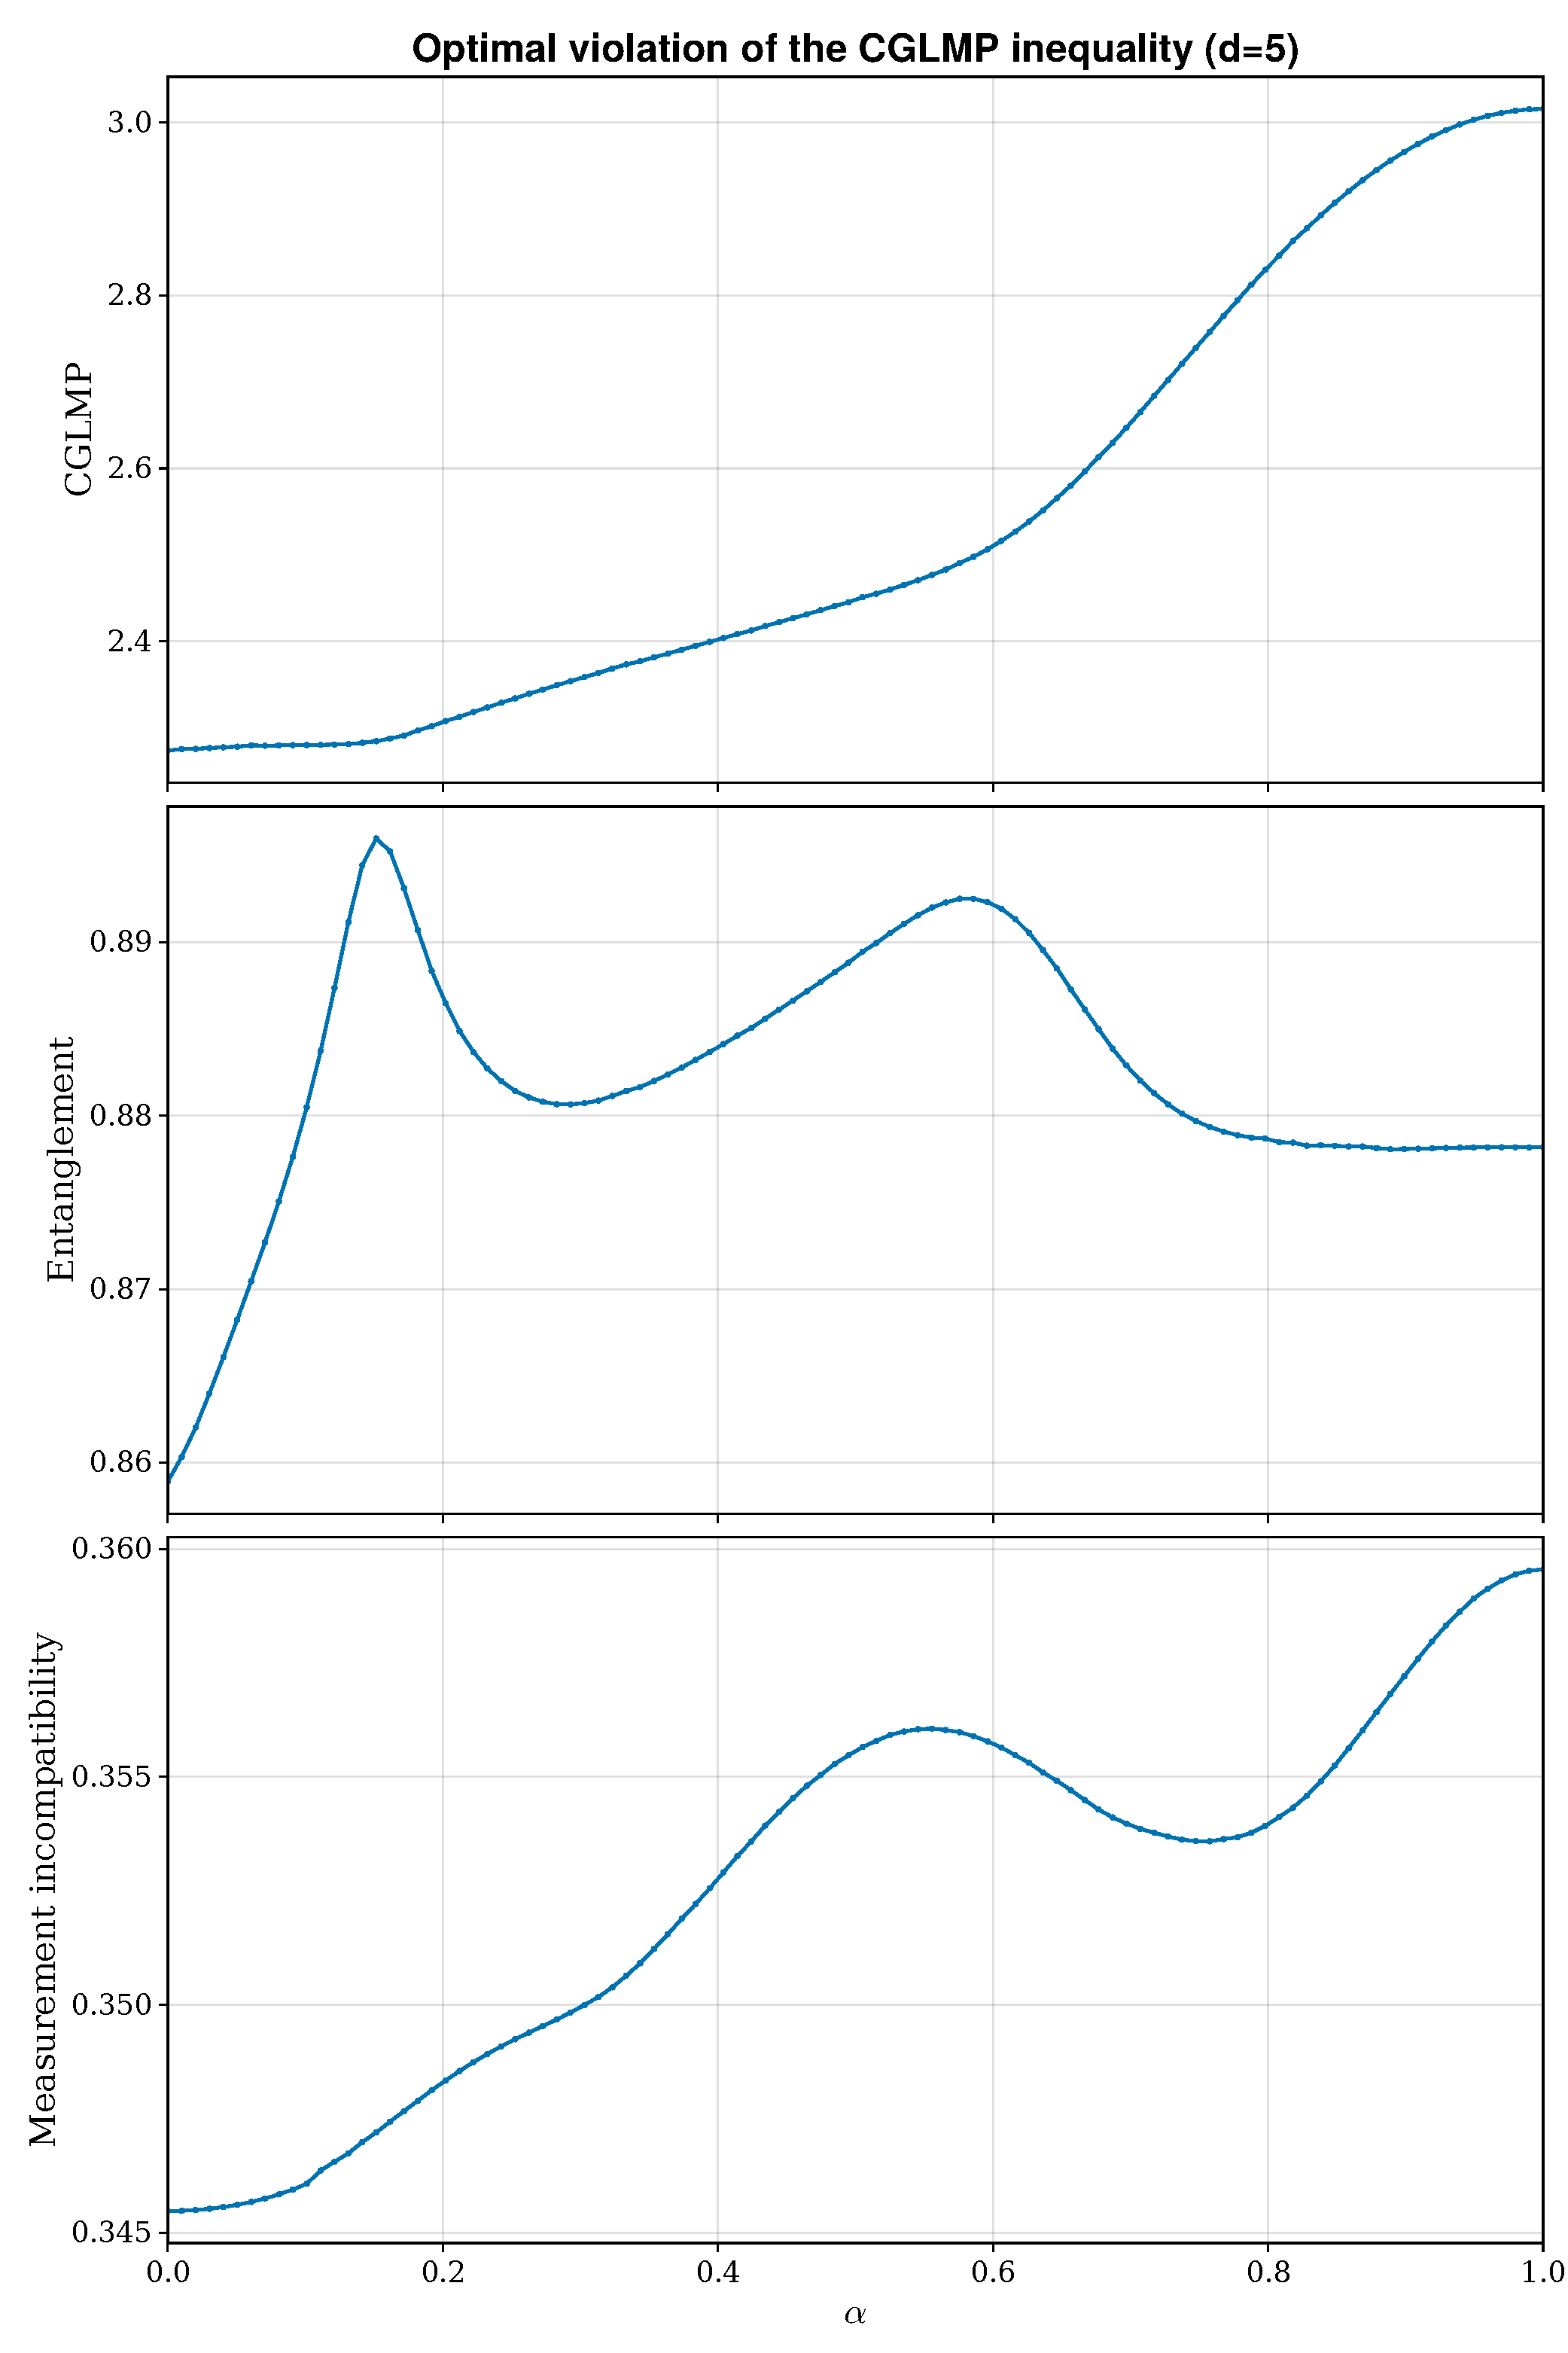
\includegraphics[width=0.6\linewidth]{resultsCGLMP/cglmp_d5.pdf}
    \caption{CGLMP inequality violation for $d=5$, and entanglement and measurement incompatibility quantifiers.}
    \label{fig:CGLMP_d5}
\end{figure}

\begin{figure}[H]
    \centering
    \includegraphics[width=0.6\linewidth]{resultsCGLMP/cglmp_d6.pdf}
    \caption{CGLMP inequality violation for $d=6$, and entanglement and measurement incompatibility quantifiers.}
    \label{fig:CGLMP_d6}
\end{figure}

\begin{figure}[H]
    \centering
    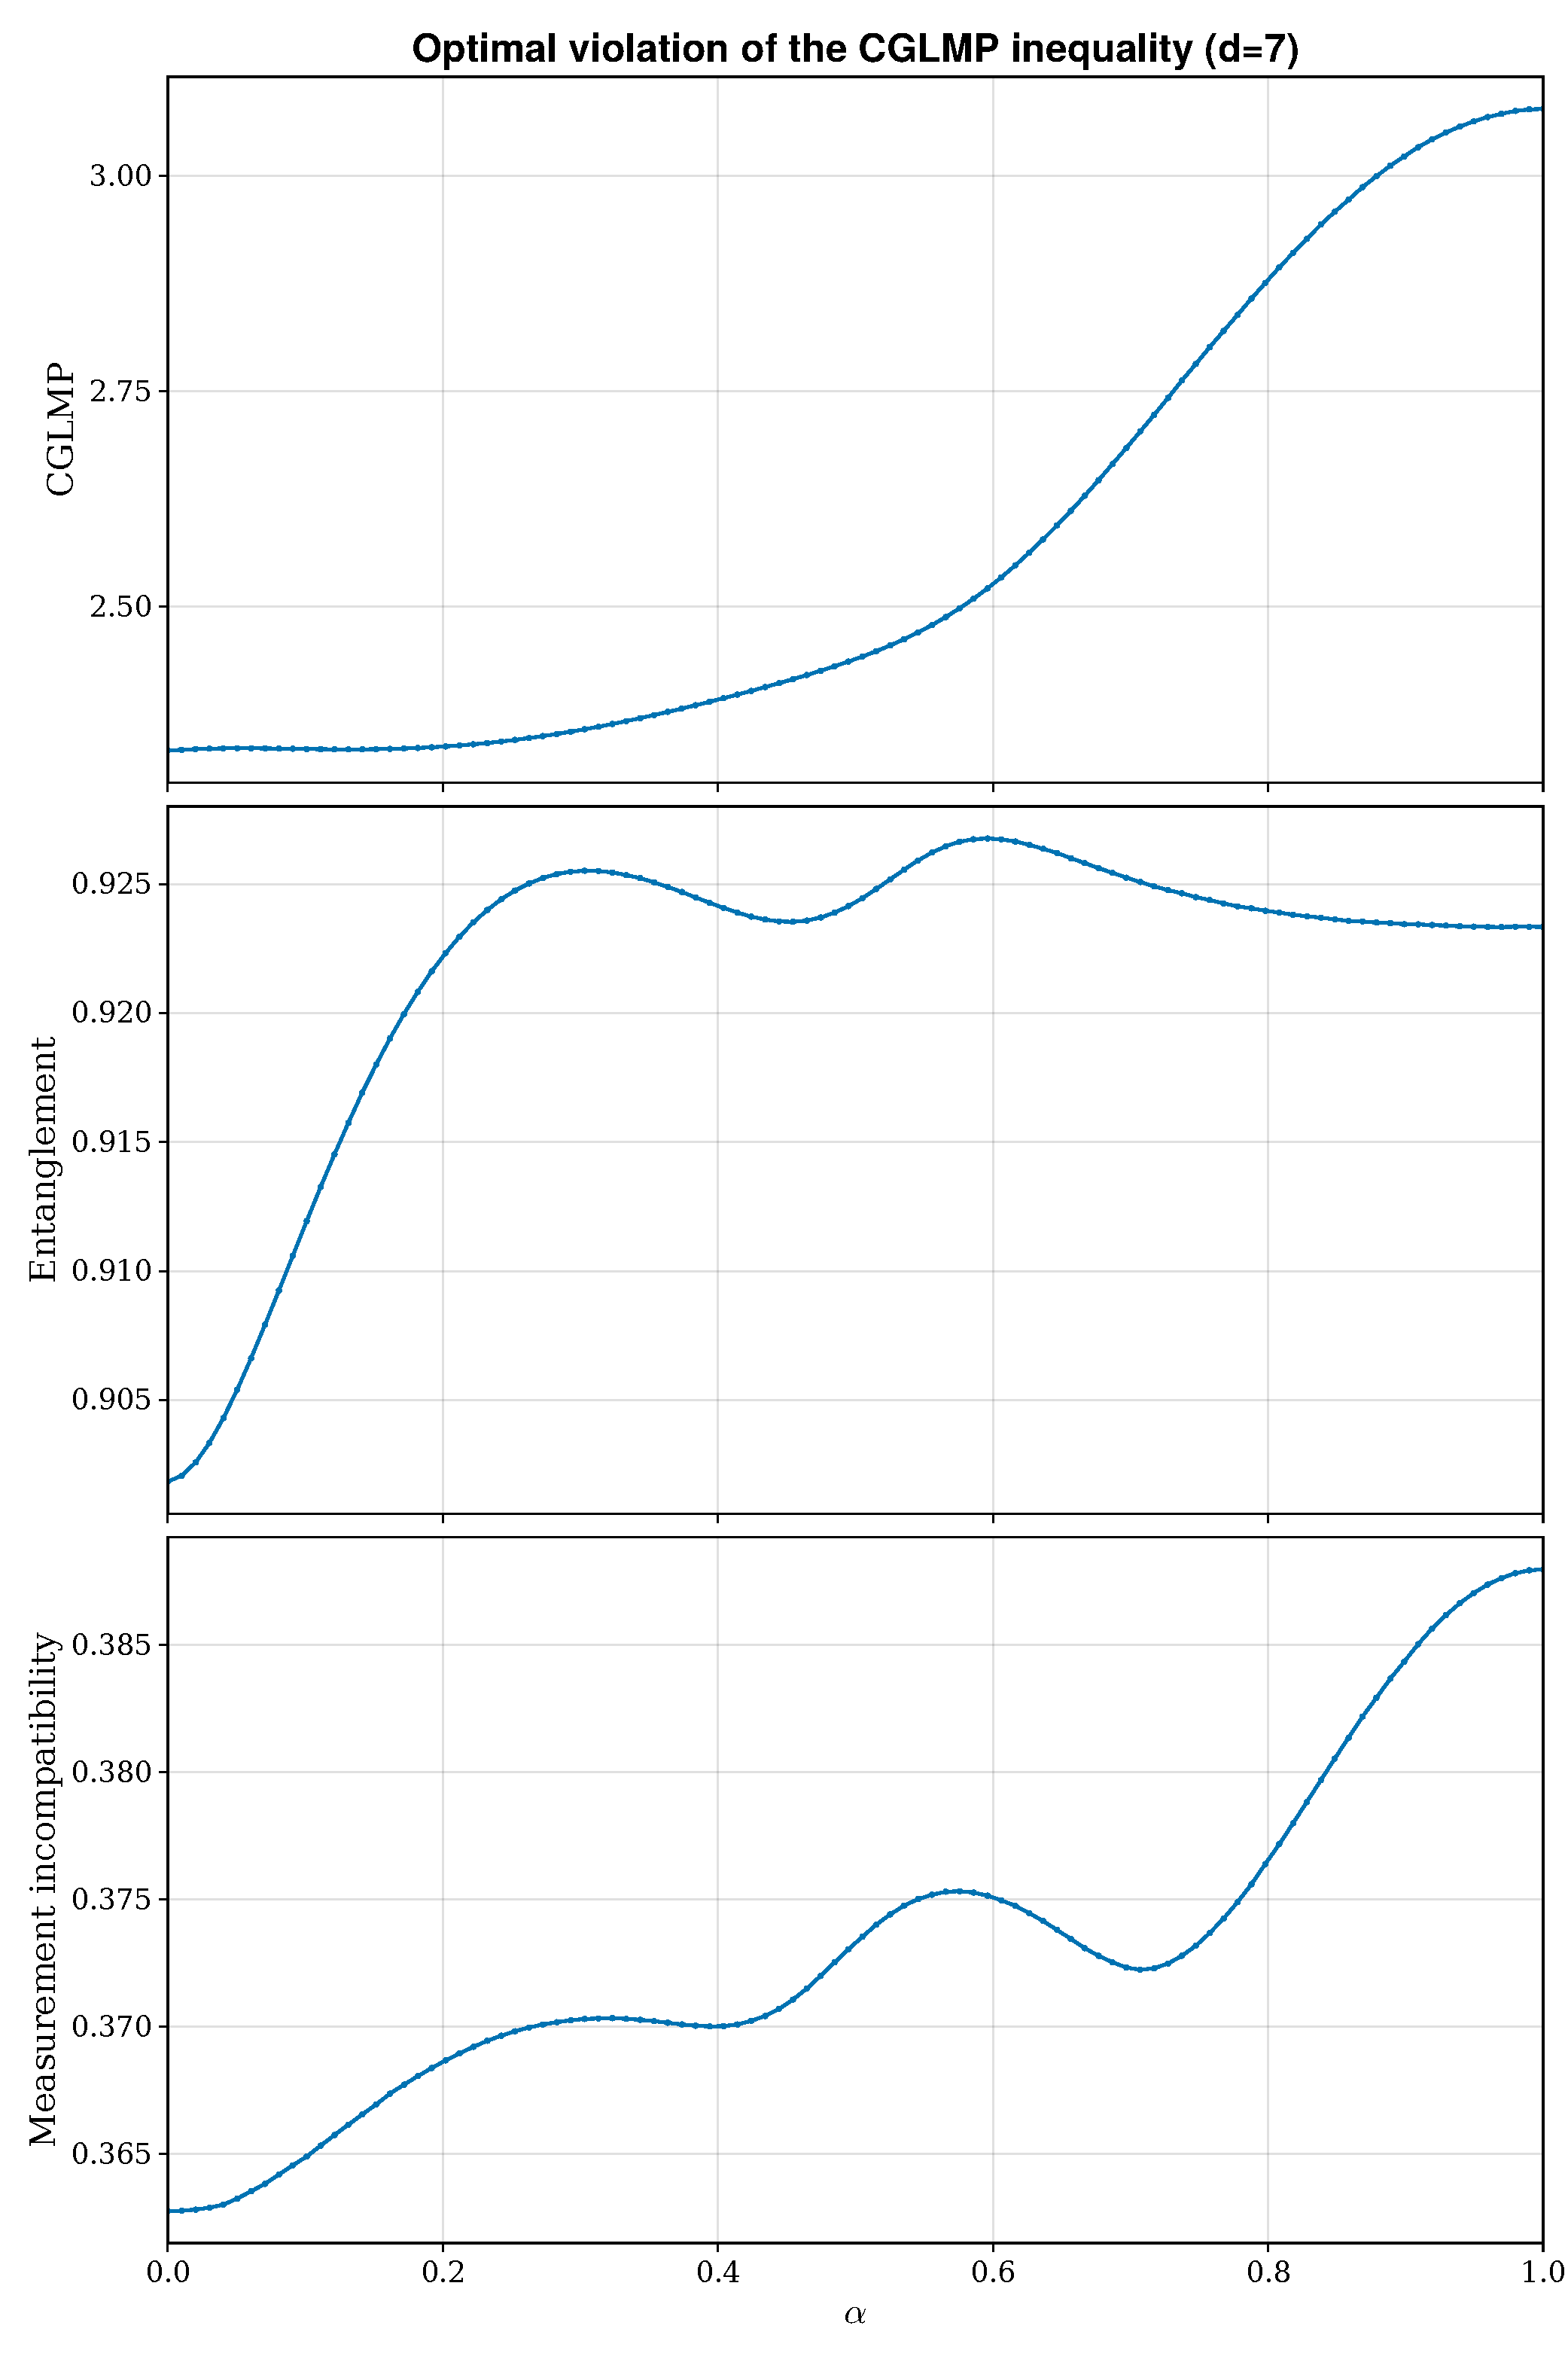
\includegraphics[width=0.6\linewidth]{resultsCGLMP/cglmp_d7.pdf}
    \caption{CGLMP inequality violation for $d=7$, and entanglement and measurement incompatibility quantifiers.}
    \label{fig:CGLMP_d7}
\end{figure}

\begin{figure}[H]
    \centering
    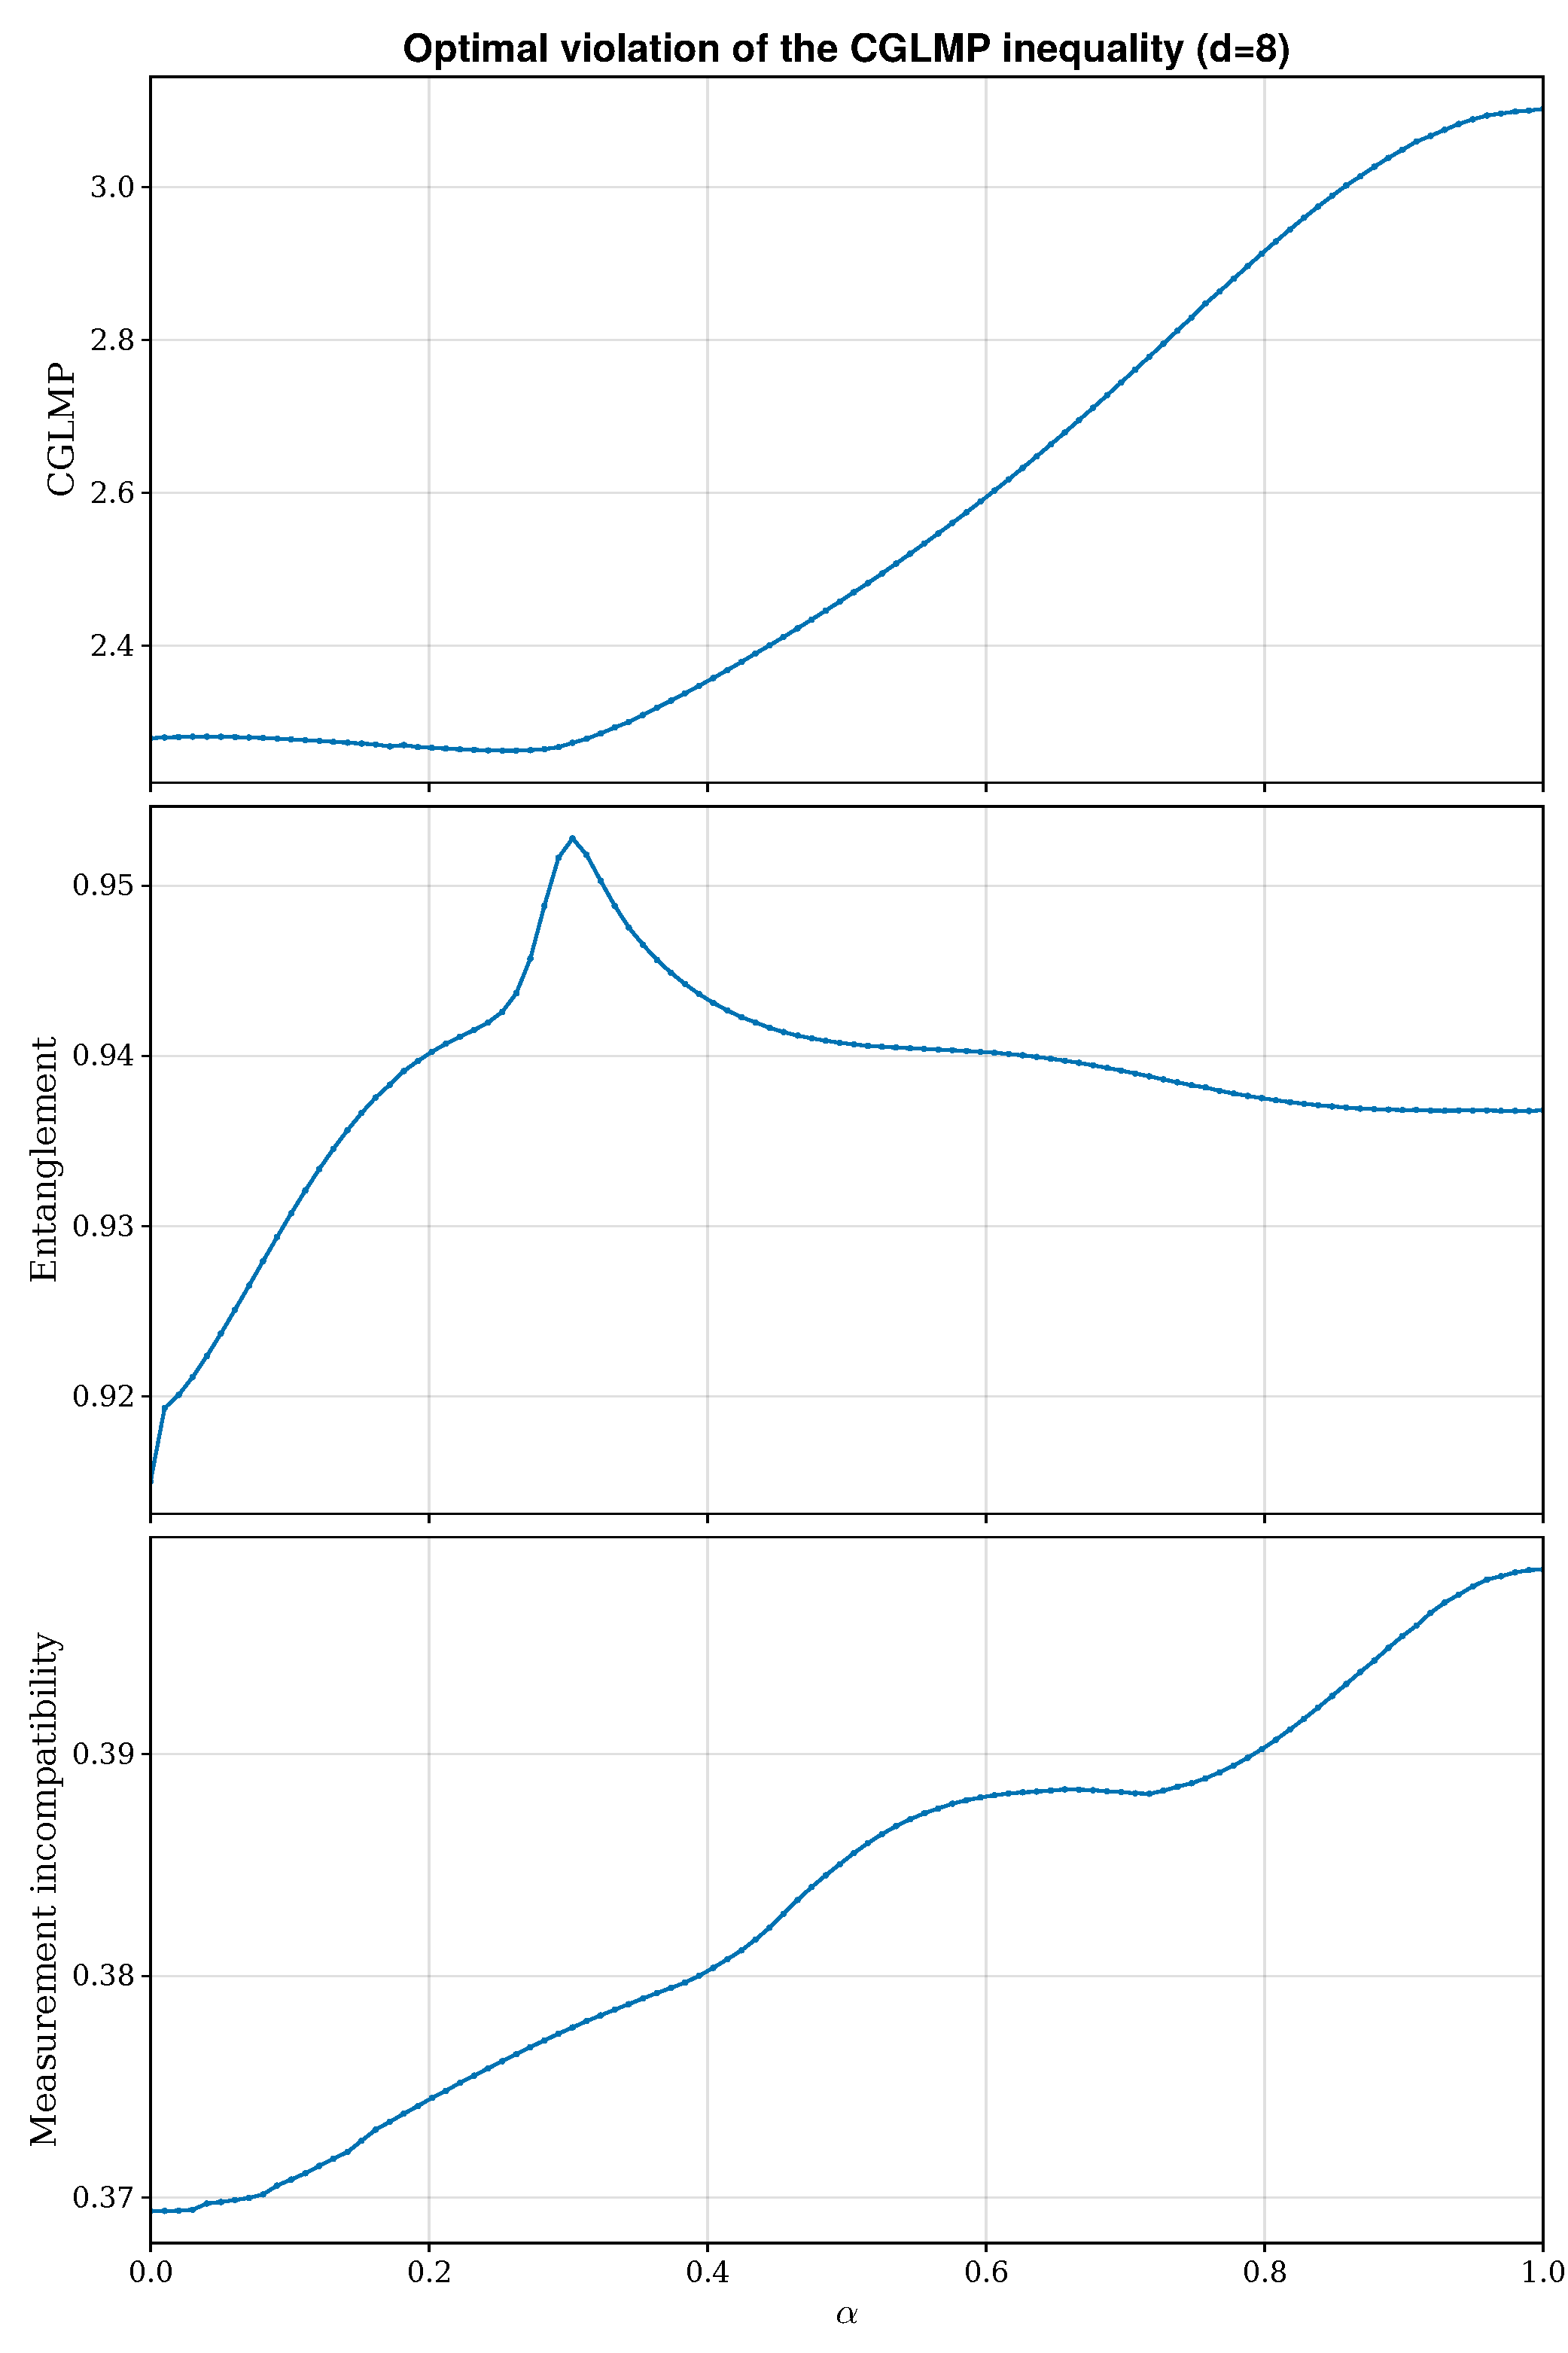
\includegraphics[width=0.6\linewidth]{resultsCGLMP/cglmp_d8.pdf}
    \caption{CGLMP inequality violation for $d=8$, and entanglement and measurement incompatibility quantifiers.}
    \label{fig:CGLMP_d8}
\end{figure}

\begin{figure}[H]
    \centering
    \includegraphics[width=0.6\linewidth]{resultsCGLMP/cglmp_d9.pdf}
    \caption{CGLMP inequality violation for $d=9$, and entanglement and measurement incompatibility quantifiers.}
    \label{fig:CGLMP_d9}
\end{figure}

\begin{figure}[H]
    \centering
    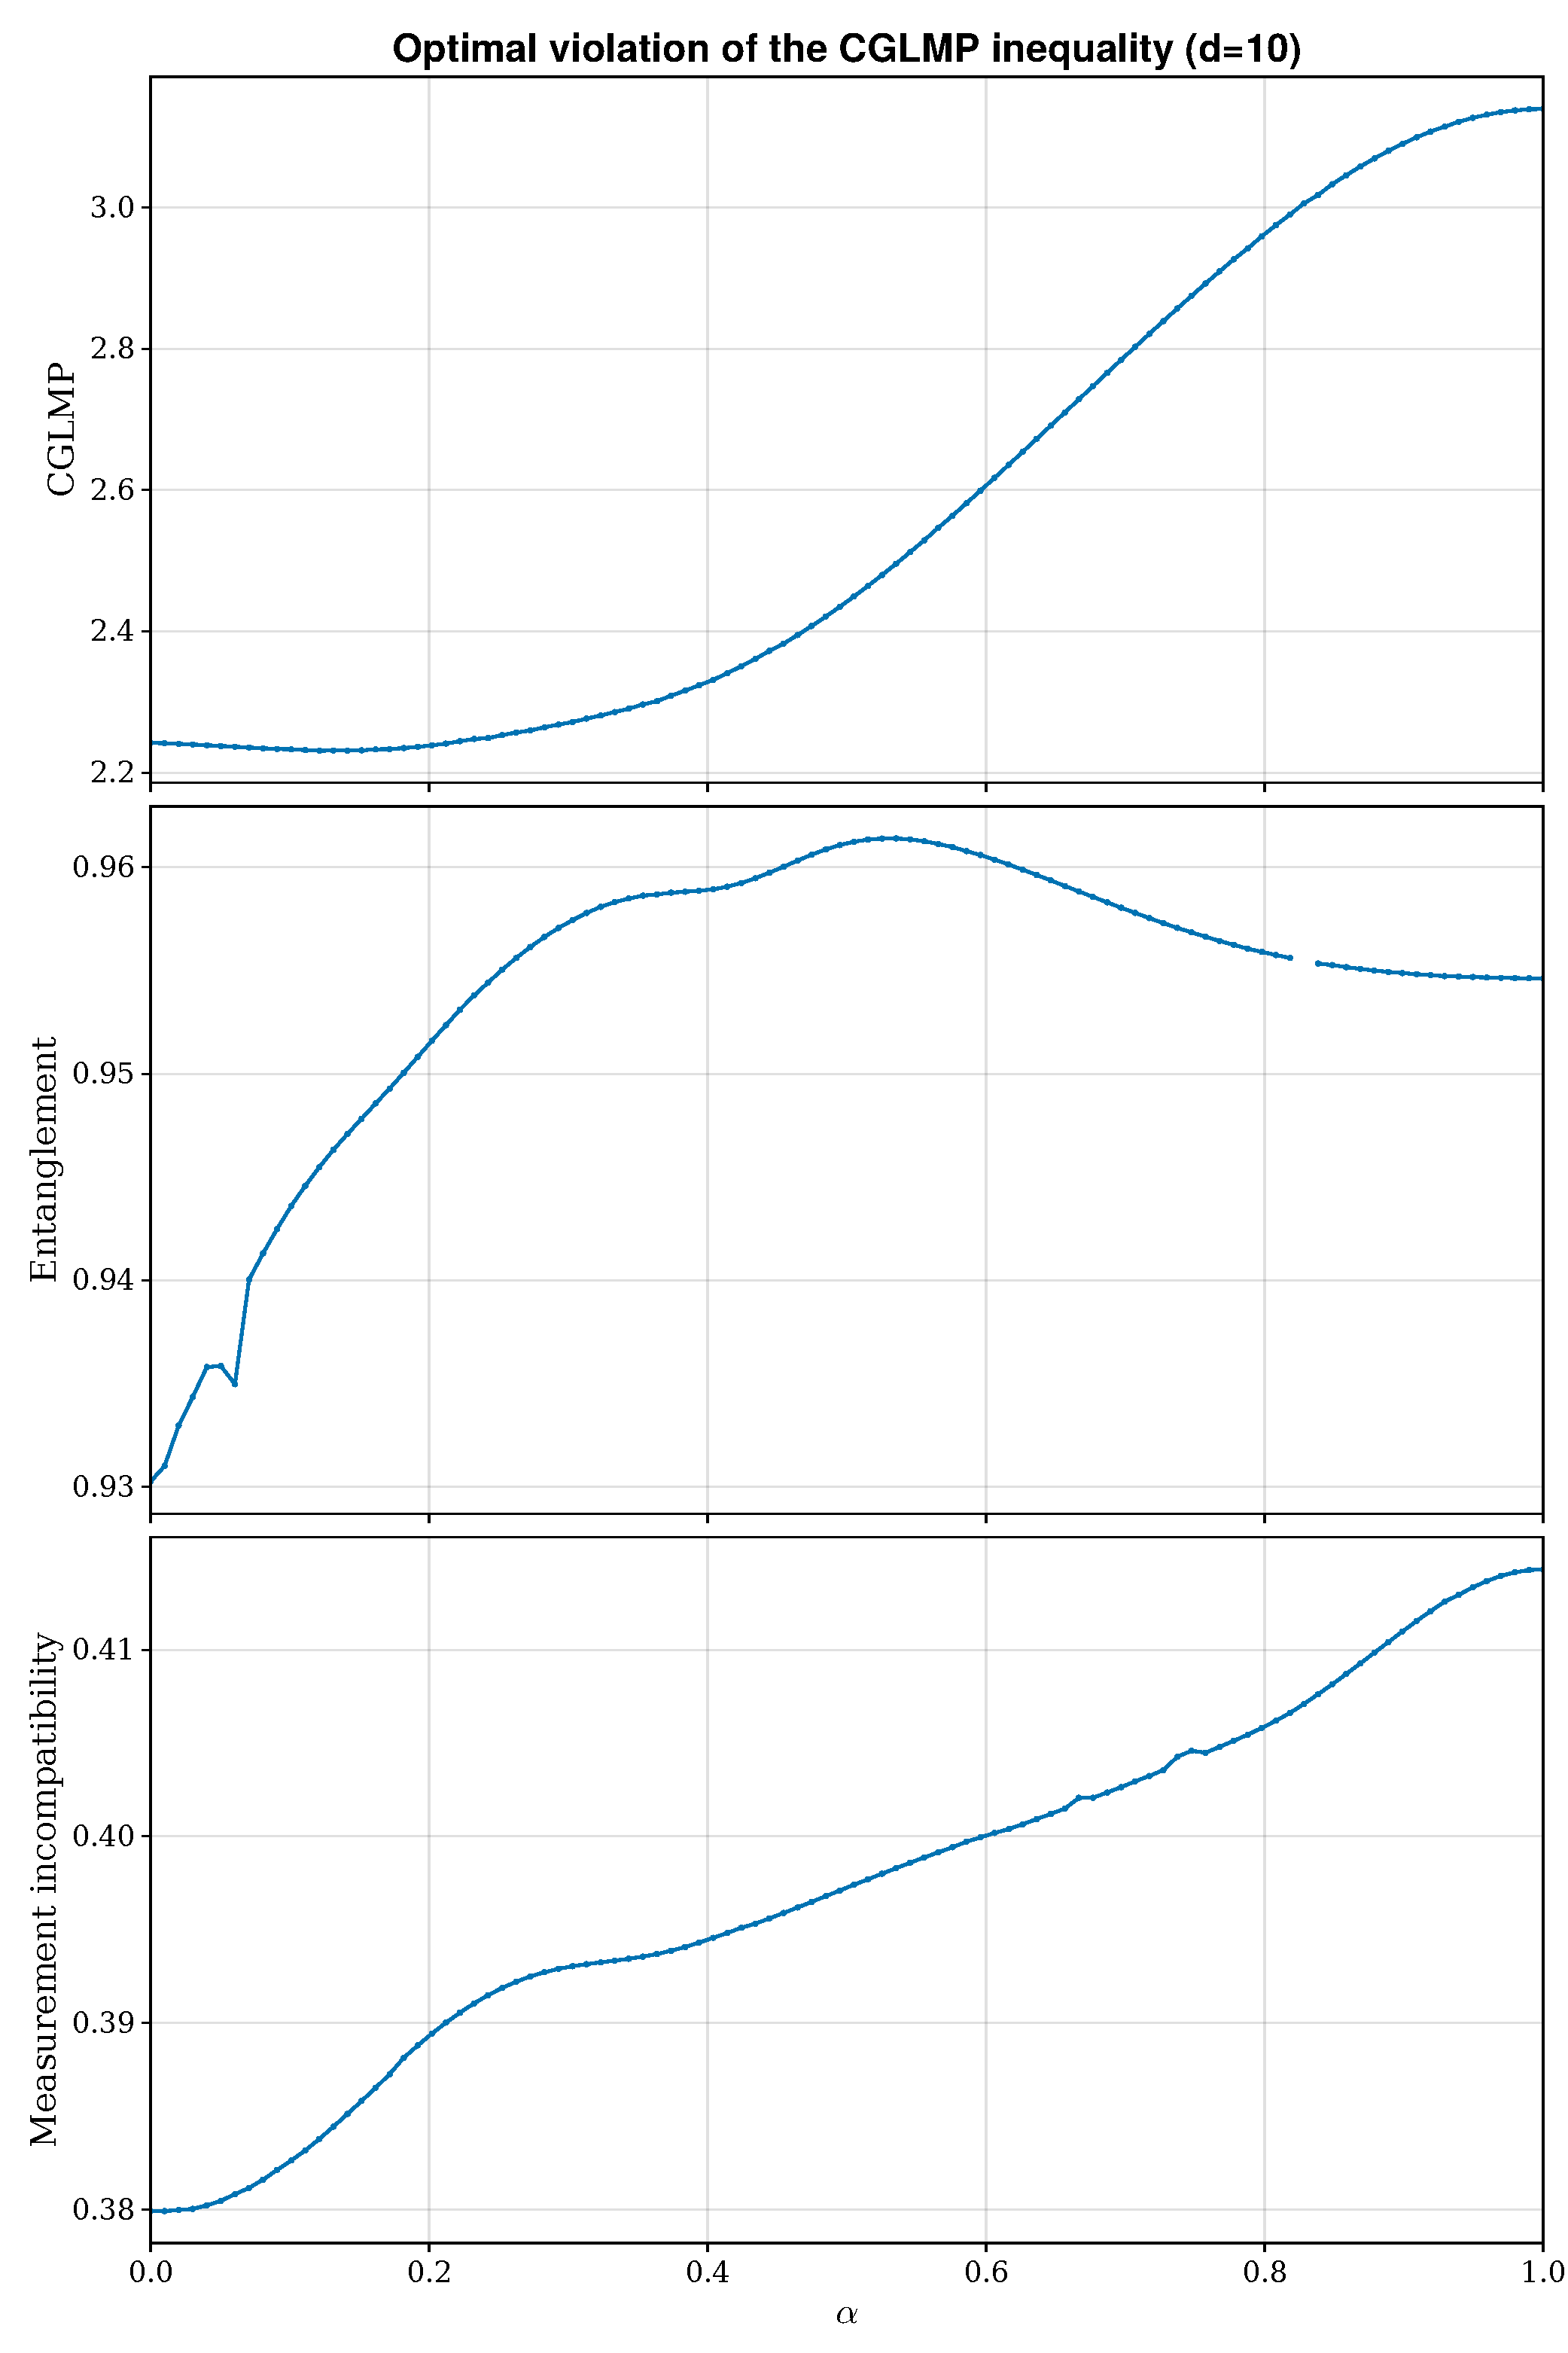
\includegraphics[width=0.6\linewidth]{resultsCGLMP/cglmp_d10.pdf}
    \caption{CGLMP inequality violation for $d=10$, and entanglement and measurement incompatibility quantifiers.}
    \label{fig:CGLMP_d10}
\end{figure}



\newpage
\printbibliography

\end{document}


